
\FloatBarrier
\section*{Introduction}
The basal nucleus of the amygdala (BA) plays a central role in context-dependent fear associations~\cite{Herry2008}, and computational modeling constitutes an important tool to understand the mechanisms involved. A neural network model of the basal amygdala could be used to simulate the differential recruitment of two distinct subpopulations of neurons during conditioning and extinction of fear memory~\cite{Vlachos2011}. Differential activation of neurons may result from the simultaneous association of the conditioned and unconditioned stimuli ($CS-US$) in the conditioning context, and weakened association in the extinction context. For a specific context, neurons are stimulated by different contextual inputs ($CTX$)~\cite{Herry2008}. Vlachos et al.~\cite{Vlachos2011} developed two models to study this dynamics in the BA: a mean-field model and a large-scale network of leaky integrate-and-fire (LIF) neurons with conductance-based synapses. The original implementation used MATLAB for the mean-field model and the NEST simulator~\cite{Gewaltig:NEST} for the spiking network model. Here, we reimplemented the models using Python and the Brian 2 simulator~\cite{Stimberg2019}, and provided information about parameter values and simulation conditions not explicitly described in the main article. 

\FloatBarrier
\section*{Methods}
In the present work we replicate the main results from  Vlachos et. al.~\cite{Vlachos2011}. In this section, we explain the details of the implementations of the two models. We start by describing the mean-field model, then we move to the spiking network model and the measures and methodological procedures adopted in the original work. Here, we refer to the $CS-US$ input as only $CS$, since there is no explicit distinction between them in the reference work. 

\subsection*{Mean-field model}\label{sec:ratemodel}

The mean-field model is described by a Wilson-Cowan type rate dynamics~\cite{wilson1972excitatory}, and consists of two neural populations with dynamics described by

\begin{equation}
    \tau_{i}\frac{dR_{i}}{dt} = -R_{i} + \xi(t) + (k_{i}-r_{i}R_{i})\Phi(I_{i}),
    \label{eq:rate_model}
\end{equation}

\noindent where the subindex $i$ ($i \in \{\text{A},\text{B}\}$) indicates the neural population, $R_{i}$ is the time-dependent population firing rate, $\xi$ is a Gaussian white noise input $\xi(t) = \mathcal{N}(\mu, \sigma)$, $k_i$ is the maximum firing rate, $r_i$ is the refractoriness parameter, and $\Phi$ is the transfer function defined by

\begin{equation}
    \Phi(x) = \frac{1}{1 + e^{-p(x-\theta)}}.
    \label{eq:transfer_function}
\end{equation}

%\textcolor{red}{REVER FRASE: The parameters $p$, and $\theta$ control the steepness, and the value where $\Phi = 0.5$, respectively.} 
\noindent The function in Equation~\ref{eq:transfer_function} is a sigmoid with values in the range $[0, 1]$, and the parameters $p$ and $\theta$ determine its steepness and point of maximum slope, respectively. 
%$\theta$ is the position of its maximum slope. 
The input received by population $i$ is represented by $I_i$, and consists of synaptic and external inputs,

\begin{equation}
    I_{i} = \underbrace{w_{ij}R_{j}}_{\text{synaptic}} + \underbrace{w_{\rm i,CS}CS_{i} + w_{\rm i,CTX}CTX_{i}}_{\text{external}},
    \label{eq:inputs}
\end{equation}

\noindent where, $w_{ij}$ indicates the weight of the synaptic connection from population $j$ to $i$. $CS_{i}$ and $CTX_{i}$ are the conditioning and contextual inputs to population $i$ with their respective synaptic weights $w_{\rm i,CS}$ and $w_{\rm i,CTX}$.

The $CS$ input consists of a sequence of short square pulses of 50 ms duration each, and the $CTX$ input is a longer square pulse applied continuously.
%step function that lasts for the whole simulation. 
When $CTX$ is active for population $i$ it is silent for population $j$ and vice-versa (see Figure~\ref{fig:esquema_rate}).

The weight $w_{\rm i,CTX}$ is fixed but the weight $w_{\rm i,CS}$ varies with time according to the following learning rule
\begin{equation}
    \frac{dw_{\rm i,CS}}{dt} = \alpha_{i}CS\text{ }CTX_{i},
    \label{eq:learning_rate}
\end{equation}

\noindent where $\alpha_{i}$ is the learning rate. All parameters used in the simulations of the mean-field model are shown in Table~\ref{tab:rate_model}.

\begin{table}[!h]
\caption{Parameters of the mean-field model (Equations~\ref{eq:rate_model}-~\ref{eq:learning_rate}) used in our simulations.}
\centering
\begin{tabular}{llr@{~}l}
\hline
\multicolumn{4}{c}{Rate model parameters}                   \\ \hline
Steepness of $\Phi$          & $p$        & 1.2 & s \\
Maximum slope of $\Phi$             & $\theta$        & 2.8 & Hz \\
Maximum firing rate                & $k_i$        & 0.97 & Hz \\
Refractoriness parameter & $r_i$    & $10^{-3}$ &   \\
Learning rate & $\alpha$    & 0.15 & s \\
$CS$ input strength         & $CS$        & 0.5 \\
$CTX$ input strength          & $CTX_{A,B}$        & 0.3 \\
 $CTX$ synaptic weight           & $w_{\rm CTX}$ & 1.0 &    \\ 
 Initial $CS$ synaptic weight           & $w_{CS}$ & 1.0 &    \\ 
Population coupling synaptic weight          & $w_{ij}$ & $-1.0$ &    \\ \hline
\end{tabular}
\label{tab:rate_model}
\end{table}

\begin{figure}[!ht]
\centering
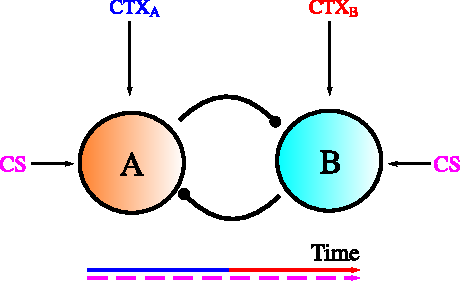
\includegraphics[width=0.6\textwidth]{figures/ratemodel.pdf}
\caption{\label{fig:esquema_rate} Schematic representation of the mean-field model. Populations $A$ and $B$ are mutually synaptically connected. The two populations receive the same $CS$ input (short pulses), and population $A$ receives a $CTX_{\rm A}$ continuous input and population $B$ receives a $CTX_{\rm B}$ continuous input. The colored time axis indicates when each of such stimuli is active. Excitatory connections are represented by arrows and inhibitory ones by circles.}
\end{figure}

%\subsection*{Neurons, network composition and connectivity}
\subsection*{Spiking network model}

Neurons of the spiking network model were described by the leaky-integrate-and-fire (LIF) model. The subthreshold dynamics of neuron $i$ is given by

\begin{equation}
\label{eq: neuron model}
\frac{dv^i}{dt} = \left ( G_l \left ( E_0-v^i \right ) + G_{exc}^i\left ( E_{exc} - v^i \right ) + G_{inh}^i\left ( E_{inh} - v^i \right ) \right )/C_m,
\end{equation}

where $v^i$ is the membrane potential, $G_l$ is the membrane (leakage) conductance, $G_{exc}$ is the total excitatory synaptic conductance, $G_{inh}$ is the total inhibitory synaptic conductance, $E_0$ is the resting potential, $E_{exc}$ is the reversal potential of the excitatory synapse, $E_{inh}$ is the reversal potential of the inhibitory synapse, and $C_m$ is the membrane capacitance~\cite{kumar2008high}. When $v^i(t)\geq \theta$, where $\theta$ is the spike threshold, the neuron emits a spike and the voltage is reset to $E_k$ and remains fixed at this value for a refractory period $\tau_{ref}$. The parameters of the neuron model in Equation~\ref{eq: neuron model} are given in Table~\ref{tab: neuron model}. In the simulations, the initial conditions of the voltages $v$ of all neurons were drawn from a normal distribution with mean $E_0$ and standard deviation 3.0~mV.  

\begin{table}[!h]
\caption{Parameters of the spiking neuron model (Equation~\ref{eq: neuron model}) used in our simulations (extracted from~\cite{kumar2008high}).}
\centering
\begin{tabular}{llr@{~}l}
\hline
\multicolumn{4}{c}{Spiking neuron parameters}                   \\ \hline
Membrane conductance          & $G_l$        & 16.7 & nS  \\
Resting potential             & $E_0$        & -70.0 & mV \\
Reset voltage                 & $E_k$        & -70.0 & mV \\
Excitatory synaptic reversal potential & $E_{exc}$    & 0.0 & mV   \\
Inhibitory synaptic reversal potential & $E_{inh}$    & -80.0 & mV \\
Membrane capacitance          & $C_m$        & 250.0 & pF \\
Spike threshold             & $\theta$        & -50.0 & mV \\
Refractory period             & $\tau_{ref}$ & 2.0 & ms   \\ \hline
\end{tabular}
\label{tab: neuron model}
\end{table}

The network is composed of 4,000 neurons, of which $N_E = 3,400$ are excitatory and $N_I = 600$ are inhibitory. The neurons are randomly connected with probabilities that depend on the types (exc or inh) of the pre- and postsynaptic cells. Synapses from a neuron onto itself (autapses) are allowed. The connection probabilities are given in Table~\ref{tab: probability connection}.      

\begin{table}[!h]
\caption{Probabilities of the four types of connections between neurons and their respective synaptic weights. The synaptic weights are drawn from normal distributions with mean $\mu$ and standard deviation $\sigma$~\cite{Vlachos2011} as indicated in the table.}
\centering
\begin{tabular}{ccccc}
\hline
Connection type & \multicolumn{2}{c}{Probability} & \multicolumn{2}{c}{Synaptic weights} \\ \hline
Excitatory to excitatory   & $p_{EE}$         & 0.01         & $\mu$ = 1.25 nS  & $\sigma$ = 0.1 nS \\
Excitatory to inhibitory   & $p_{IE}$         & 0.15         & $\mu$ = 1.25 nS  & $\sigma$ = 0.1 nS \\
Inhibitory to excitatory   & $p_{EI}$         & 0.15         & $\mu$ = 2.50 nS  & $\sigma$ = 0.1 nS \\
Inhibitory to inhibitory   & $p_{II}$         & 0.10         & $\mu$ = 2.50 nS  & $\sigma$ = 0.1 nS \\ \hline
\end{tabular}
\label{tab: probability connection}
\end{table}

The synaptic conductances obey the equations

\begin{align}
    \frac{dG}{dt} &= G_{aux}-\frac{G}{\tau_r},
    \label{eq: G}
    \\
    \frac{dG_{aux}}{dt} &= -\frac{G_{aux}}{\tau_d}+ W\delta(t-t'-D),
    \label{eq: w increased}
\end{align}

where $G$ is used to represent either $G_{\rm exc}$ or  $G_{\rm inh}$, $G_{aux}$ is an auxiliary variable, and $\tau_{r}$ and $\tau_{d}$ are the rise and the decay time constants, respectively. We will use $\tau_r=\tau_d=0.326$~ms~\cite{kumar2008high}, so that $G$ is an alpha function.

In Equation~\ref{eq: w increased}, $W$ is the synaptic weight added to the variable $G_{aux}$ at time $t$ due to a spike in the presynaptic neuron at time $t'$, and $D$ is the transmission delay from pre- to postsynaptic neuron. The value of $D$ is drawn from a normal distribution with mean $\mu = 2$~ms and standard deviation $\sigma = 0.1$~ms. The value of the synaptic weight $W$ depends on the type of synapse and is indicated in Table~\ref{tab: probability connection}.


\subsection*{Spiking network inputs}

Besides recurrent connections from other network neurons, each neuron of the spiking network model receives three kinds of input: background ($BKG$), consisting of 1,000 inputs per neuron representing external synapses received from neurons in other brain areas; conditioned stimulus ($CS$), consisting of short pulses of 50 ms of duration; and contextual input ($CTX$). All these inputs are modeled as excitatory synapses activated by independent Poisson processes with specific rates.

The rates of the $BKG$ inputs to excitatory and inhibitory neurons are distinct. These rates were adjusted so that the baseline network spiking activity was lower than 1~Hz for excitatory neurons and between 10-15~Hz for inhibitory neurons, as observed experimentally~\cite{sah2003amygdaloid}. The rates of the $CS$ and $CTX$ inputs are the same for all neurons. The input rates and their respective synaptic weights are shown in Table~\ref{tab: inputs}. 

To model conditioning and extinction of fear memories in the BA, two subpopulations of excitatory neurons containing 20\% of $N_{E}$, i.e. 680 neurons, were chosen without overlap. The first subpopulation (${pop}_A$) represents the fear neurons which receive context$_A$ input ($CTX_A$), and the second (${pop}_B$) represents the extinction neurons which receive context$_B$ input ($CTX_B$). 

\begin{table}[]
\caption{Parameters (rates of Poisson processes and synaptic weights) and types of synaptic inputs applied to the network neurons. The weights of all $BKG$ and $CS$ to $INH$ (inhibitory neurons) inputs are fixed, while the weights of the $CS$ to $EXC$ (excitatory neurons) and $CTX$ inputs are plastic and have their initial values drawn from normal distributions with parameters (mean $\mu$ and standard deviation $\sigma$) indicated in the table.}
\centering
\begin{tabular}{cccc}
\hline
\multicolumn{4}{c}{Inputs parameters}                   \\ \hline
Connection             & Type    & Rate   & Weight                             \\
$BKG$ to $EXC$         & Static  & 5 Hz   & 1.25 nS                            \\
$BKG$ to $INH$         & Static  & 6 Hz    & 1.25 nS                            \\
$CS$ to $INH$          & Static  & 500 Hz & $\mu = 0.9$ nS, $\sigma = 0.1$ nS  \\
$CS$ to $EXC$          & Plastic & 500 Hz & $\mu = 0.9$ nS, $\sigma = 0.1$ nS  \\
$CTX$ to subpop. $A/B$ & Plastic & 300 Hz & $\mu = 0.4$ nS, $\sigma = 0.05$ nS \\ \hline
\end{tabular}
\label{tab: inputs}
\end{table}

\FloatBarrier
Figure~\ref{fig:esquema_rede} shows all the inputs described above with emphasis on subpopulations A and B that are formed exclusively by excitatory neurons. The first stage of the simulation represents the conditioning phase in which $CTX_A$ and $CS$ are activated ($CTX_B$ is deactivated), and the second stage represents the extinction phase, in which $CTX_B$ and $CS$ are activated ($CTX_A$ is deactivated).

\begin{figure}[!ht]
\centering
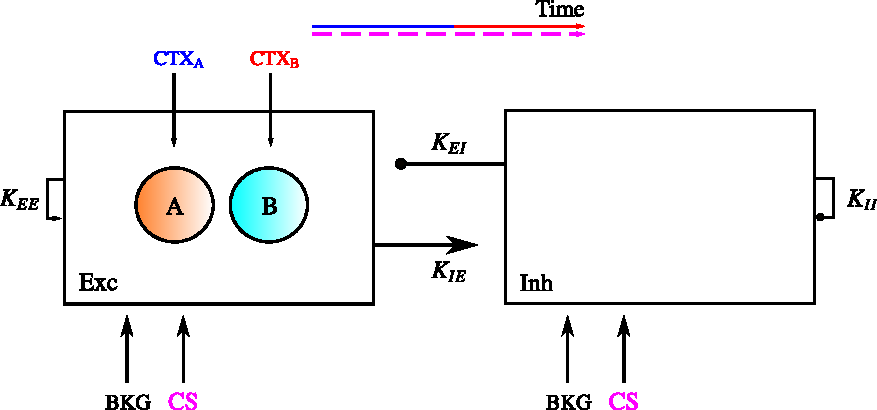
\includegraphics[width=0.8\textwidth]{figures/esquema_rate_amygdala_b.pdf}
\caption{\label{fig:esquema_rede} Schematic diagram of the spiking network model. Excitatory and inhibitory populations are represented by rectangles with the two excitatory subpopulations (A and B) that receive $CTX$ inputs highlighted as colored circles. The excitatory and inhibitory populations receive $BKG$ and $CS$ (short pulses) inputs and the subpopulations A and B receive aditional $CTX_{\rm A}$ and $CTX_{\rm B}$ inputs, respectively. The colored time axis indicates when $CTX_{\rm A}$ and $CTX_{\rm B}$ inputs are active. Excitatory connections are represented by arrows and inhibitory ones by circles.}
\end{figure}

\FloatBarrier
\subsection*{Plasticity}
The synaptic weights of all network connections are static, except the ones of the connections from the $CS$ and $CTX$ inputs to the excitatory neurons, which are modified according to the following phenomenological rule:

\begin{equation}
\label{eq: plasticity}
    w_+ = \begin{cases}
        w_- +\alpha_1 \cdot h \cdot m \cdot c \cdot\left | w_{max}-w_- \right | & \textrm{if $CS$ and $CTX$ temporally overlap}\\
        w_- -\alpha_2 \cdot m \cdot c \cdot \left | w_{min}-w_- \right | & \textrm{otherwise,}
\end{cases}
\end{equation}

where $w_-$ is the synaptic weight before the update, $w_+$ is the synaptic weight after the update, $\alpha_1$ and $\alpha_2$ are the learning rates, $w_{max}$ ($w_{mim}$) is the maximum (minimum) value of the synaptic weight, $m$ is a binary number that represents the action of a neuromodulator, and $c$ and $h$ are auxiliary variables that encode the recent activity in the synapse that receives input from $CS$ and $CTX$, respectively.

The overlap described in Equation~\ref{eq: plasticity} refers to when there is a temporal superposition of $CS$ and $CTX$ inputs for the same neuron on a time window of up to 100~ms. If the temporal overlap occurs, the synapses that connect the $CS$ and $CTX$ to the target neuron are strengthened; otherwise, both synapses are weakened. 
%Note that this rule for plasticity is somewhat peculiar because it depends only on the temporal correlations between the two presynaptic inputs ($CS$ and $CTX$).

The dynamics of the variables $c$ and $h$ are described by

\begin{align}
    \dot{c} &= - \frac{c}{\tau_c} + c_u \cdot \delta(t - t_{pre-CS})
    \label{eq: c}
    \\
    \dot{h} &= - \frac{h}{\tau_h} + h_u \cdot \delta(t - t_{pre-CTX}),
    \label{eq: h}
\end{align}

where $\tau_c$ and $\tau_h$ are time constants and $c_u$ ($h_u$) is an increase in variable the $c$ ($h$) when a spike is emitted by the $CS$ ($CTX$) source at $t = t_{pre}$. The values of the parameters used to model synaptic plasticity are shown in Table~\ref{tab: synaptic plasticity}.


\begin{table}[t]
\centering
\caption{Synaptic plasticity parameters}
\begin{tabular}{lcc}
\hline
\multicolumn{3}{c}{Synaptic plasticity}                                                                                                                          \\ \hline
Learning rates                                                                                                          & $\alpha_1$, $\alpha_2$ & $1.6 \times 10^{-3}$ \\
Neuromodulator present/absent                                                                                           & $m$                    & 0 or 1        \\
Maximum value of synaptic weight                                                                                        & $w_{max}$              & 4.0 nS        \\
Mininum value of synaptic weight                                                                                        & $w_{min}$              & 0.4 nS        \\
Time constant for variable $c$                                                                                          & $\tau_c$               & 10 ms         \\
Time constant for variable $h$                                                                                          & $\tau_h$               & 10 ms         \\
\begin{tabular}[c]{@{}c@{}}Increment to variable $c$ \end{tabular}   & $c_u$                  & 0.35          \\
\begin{tabular}[c]{@{}c@{}}Increment to variable $h$ \end{tabular} & $h_u$                  & 0.35          \\ \hline
\end{tabular}
\label{tab: synaptic plasticity}
\end{table}

\FloatBarrier
\subsection*{Simulation protocols}

In this section we define the protocols used for the simulations of the spiking network model. In all cases described below, the $BGK$ input is always active.

\subsubsection*{Spontaneous Activity}
The network was simulated only with the $BKG$ input during 1 second to evaluate the spontaneous activity generated by the model.

\subsubsection*{Dynamics of conditioning and extinction processes}
After 50~ms of initial transient period, the conditioning phase begins with the activation of the input $CTX_A$ and the application of 5 $CS$ pulses (50~ms each) intercalated at intervals of 150~ms. After $CTX_A$ is turned off, a transient period of $100$~ms follows and the same protocol is repeated for $CTX_B$ but with 6 $CS$ pulses instead of 5.

During each presentation of $CS$ (both in the conditioning phase and in the extinction phase), the variable $m$ in Equation~\ref{eq: plasticity} takes the value 1, and otherwise the value 0. Thus, the synaptic weights $CS$ and $CTX$ vary during the simulation due to synaptic plasticity, starting with the initial values given in Table~\ref{tab: inputs}.

\subsubsection*{Fear renewal} The fear renewal stage starts by repeating the previous protocol followed by the reactivation of $CTX_A$ at the end of the extinction phase, together with a single presentation of the $CS$. 

\subsubsection*{High connectivity introduces gamma oscillations}
In this protocol the $p_{ii}$ (see Table~\ref{tab: probability connection}) is increased from 0.1 to 0.5 and only the conditioning phase is activated with the application of 10 $CS$ pulses.

\subsubsection*{Blockage of inhibition}
This protocol follows the same procedure described in \textit{Dynamics of conditioning and extinction processes}, but two different conditions are simulated: either 50\% or 90\% of inhibitory neurons are deactivated during the extinction phase.

\subsection*{Measures}\label{sec:measures}
In this section we show how the measures used in our replication of the original study are defined:

\begin{itemize}
    \item Throughout the simulation, we recorded the firing times for the construction of raster plots of neuronal activity.
    
    \item During $CS$ presentations to $pop_A$ and $pop_B$, we counted the total number of spikes in each subpopulation and divided it by the $CS$ duration (50~ms) to calculate the average firing rate.
    
    \item We recorded the time series of $CS$ and $CTX$ synaptic strengths to $pop_A$ and $pop_B$ throughout the simulations. With that, we calculated the averages of these weights separately during each presentation of $CS$.
    
    \item The population spiking activity is the average spike count within a time window $\Delta t = 1$ ms, unless otherwise stated.
    
    \item We estimated the power spectrum density ($PSD$) of the population spiking activity using the Welch's method (from python package \textit{SciPy}).
    
    \item The synchrony index was calculated as the variance of the population spiking activity divided by its mean. This measure is a simplification of the normalized synchrony index introduced by Golomb and Rinzel~\cite{Golomb1993, Golomb2007}.
    
\end{itemize}

\subsection*{Important information needed during replication}
The general information necessary for the replication done here was available in the original article. However, some details were not found neither in the reference paper nor in the supplementary material. Here we list these details and describe the considerations we made to replicate the results.

\subsubsection*{Missing parameter values}
\begin{itemize}

    \item Almost every parameter for the mean-field model is not present in the original work, namely the strength of the $CS$ and $CTX$ inputs, $w_{ij}$, and $w_{\rm CTX}$.
    
    \item The values of the spiking neuron parameters $\tau_m$, $E_0$, $E_{exc}$, $E_{inh}$, $\theta$ and $E_K$ in Equation 5 are said to be given in Table S1F of the supplementary material of the reference~\cite{Vlachos2011} paper. However, the only parameter value given in Table S1F is the one of $\tau_{ref}$. The value of $\theta$ is given in the caption of Figure 5 as $-57$ mV and the other are missing. Furthermore, the initial value of $v$ is not mentioned.
    
    \item The synapse model used is defined in the main text only as a conductance-based synapse with no mention to the conductance dynamics. Looking at the supplementary material, we found that the conductance time-course was described by a difference of exponentials. The equation is described in Table S1G~\cite{Vlachos2011} but is not cited in the main text. Nevertheless, the values of the parameters $\tau_r$, $\tau_d$ and $t_{peak}$ are not given.
    
    \item Some parameters are also not given in the main text for the synaptic plasticity model described by equations 6-8. These parameters are: $w_{max}$, $w_{min}$, $A$, $B$, $\tau_c$ and $\tau_h$.
    %Although Table S1E from supplementary material~\cite{Vlachos2011} give us the synaptic weight of plastic connections as a normal distribution, the definition of $w_{max}$ induce the understanding that it is a constant value.
    Moreover, but less important, parameters $\alpha_1$ and $\alpha_2$ are written in Table S1H as $a_1$ and $a_2$.
    
    \item Table S1I from the supplementary material~\cite{Vlachos2011} defines $BKG$ current injections to excitatory and inhibitory neurons) with DC and AC amplitude values. However, there is no information about the frequency or phase for the AC currents. 
    
    \item In Figures 5, 7, and 8 of the original work~\cite{Vlachos2011}, the authors used spike activity histograms to obtain the firing rate time series that characterize the population activity. However, the bin sizes used are different and not informed.
   
   \item The \textit{High connectivity introduces gamma oscillations} protocol adopted in the original article was not clear if only the conditioning phase was considered, and the number of $CS$ presentations was not specified.
    
\end{itemize}

\subsubsection*{Approximations done to replicate the results}
\begin{itemize}

    \item In the mean-field model we considered the inputs $CS$ and $CTX_{A/B}$ as square pulses with the same heights as used for the spiking network model ($500$ and $300$~Hz, respectively), but we divided them by $1000$ so that they remain below 1. We considered the synaptic weights as unitary, i.e., $w_{i,CS} = w_{i,CTX} = -w_{ij} = 1$.
    
    \item The neuron model equation used in the original text (Equation 5 of~\cite{Vlachos2011}) has a dimensional inconsistency. By reviewing the references cited by the authors, we found our Equation~\ref{eq: neuron model} in reference~\cite{kumar2008high}, which describes the same neuronal dynamics. We adopted this equation here with the same parameters given in~\cite{kumar2008high} and shown in Table~\ref{tab: neuron model}.
    
    \item The description of the synaptic model was also extracted from reference~\cite{kumar2008high}, where the synaptic conductances are given by a difference of exponentials with $\tau_r = \tau_d = 0.326$~ms. To implement the difference of exponentials in Brian 2, it was necessary to use two ordinary differential equations as shown in Equations~\ref{eq: G} and~\ref{eq: w increased}.
    
    %\item \textcolor{red}{Since we did not have the parameters of the synaptic conductance dynamics, to simplify and have less parameters to estimate we used a synaptic conductance with an exponential decay. No strong reasons were stated for using alpha synapses in the reference.}
    
    \item Due to the lack of details on the application of AC and DC currents to model the $BKG$ input, we opted for the use of Poisson train generators (Table~\ref{tab: inputs}), which promoted a spontaneous activity compatible with what was experimentally expected~\cite{sah2003amygdaloid}.
    
    \item To replicate the results obtained in the evolution of synaptic weights, we used the values of $CS$ and $CTX$ shown in Table~\ref{tab: inputs}, which differ from those described in the supplementary material of the reference article~\cite{Vlachos2011}.
    
    \item In Equations~\ref{eq: c} and~\ref{eq: h}, we named the parameters $c_u$ and $h_u$ instead of $A$ and $B$ as in the reference article~\cite{Vlachos2011} to avoid misunderstandings in relation to subpopulations A and B. We also specified in these equations $t_{pre-CS}$ and $t_{pre-CTX}$, which indicate when increments in auxiliary variables occur.
    
    \item In assessing how the increase in network connectivity introduces gamma oscillations, the authors did not clearly show how the frequency of population activity and the synchrony index were determined. In our replication, we used $PSD$ to check the frequency of oscillations in the spiking activity of the network and chose population Fano Factor as the synchrony index.
    
    \item In Figure~\ref{fig:gamma}, we used $10$ $CS$ presentations which was the minimum number of presentation necessary to reproduce the original result. 
    
\end{itemize}


\FloatBarrier
\section*{Results}
In this section, we present the results obtained from our simulations as described in Methods, which qualitatively reproduce the main results of the reference article.

\subsection*{Mean-field model}

Despite the lack of information provided by the authors for this model, we have reproduced qualitatively the expected dynamics for the conditioning and extinction phases as shown in Figure~\ref{fig:rate_model_result}\textbf{A}.% where we show the population rates for each $CS$ application.

The external inputs $CS$ and $CTX$ were generated beforehand for the whole simulation time (Figure~\ref{fig:rate_model_result}\textbf{C}). Therefore, we studied the evolution of the synaptic weights $w_{A/B,CS}$ by simply using the stimuli arrays and Equation~\ref{eq:learning_rate} without simultaneously simulating the inputs. The synaptic weights evolution in Figure~\ref{fig:rate_model_result}\textbf{B} is in accordance with what was reported in the reference paper (Figures 4C-D of~\cite{Vlachos2011}).


\begin{figure}[!ht]
\centering
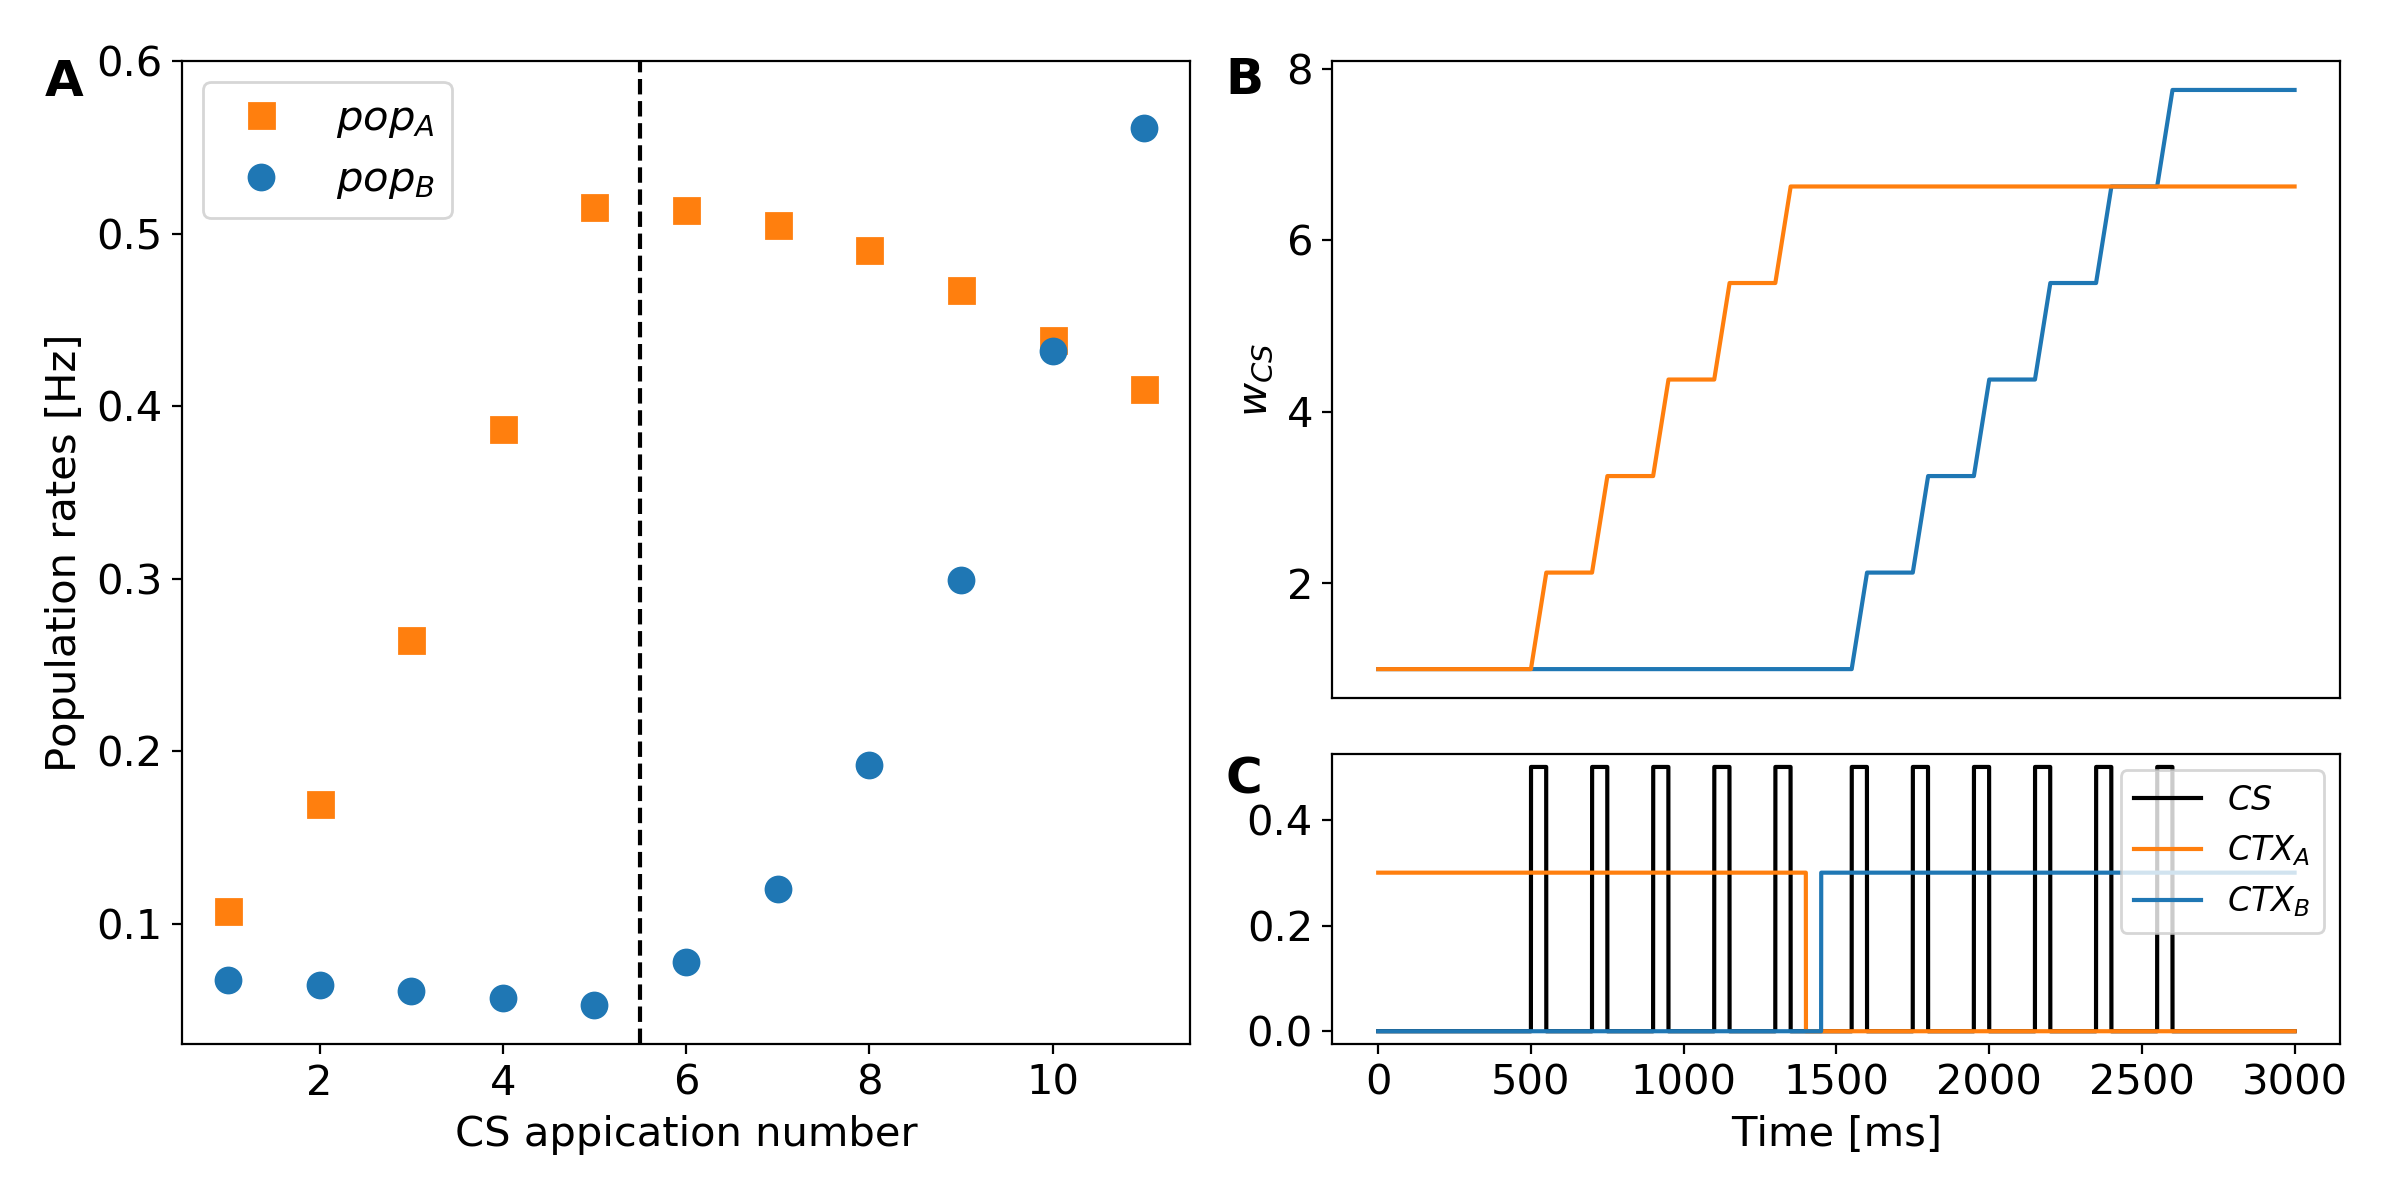
\includegraphics[width=1\textwidth]{figures/result_mean_field_model.png}
\caption{Dynamics of the mean-field model.(\textbf{A}) Firing rates of $pop_A$ and $pop_B$ at each $CS$ application. The vertical red dashed line marks the transition from application of $CTX_{\rm A}$ to $CTX_{\rm B}$. (\textbf{B}) Time evolution of $w_{A,CS}$, and $w_{B,CS}$. (\textbf{C}) Time evolution of the external inputs $CS$, $CTX_{A}$, $CTX_{B}$. \label{fig:rate_model_result}}
\end{figure}
\FloatBarrier

\subsection*{Spiking neuron network model of BA}

\subsubsection{Spontaneous Activity}

In Figure~\ref{fig:BKG} we show the raster plot of the simulated spontaneous activity of the network. The firing rates measured were 0.03 and 10.54 Hz per neuron for the excitatory and the inhibitory populations, respectively. This is compatible with the firing rates observed experimentally~\cite{sah2003amygdaloid}. This consistency test was not presented in the original work.

\begin{figure}[!ht]
\centering
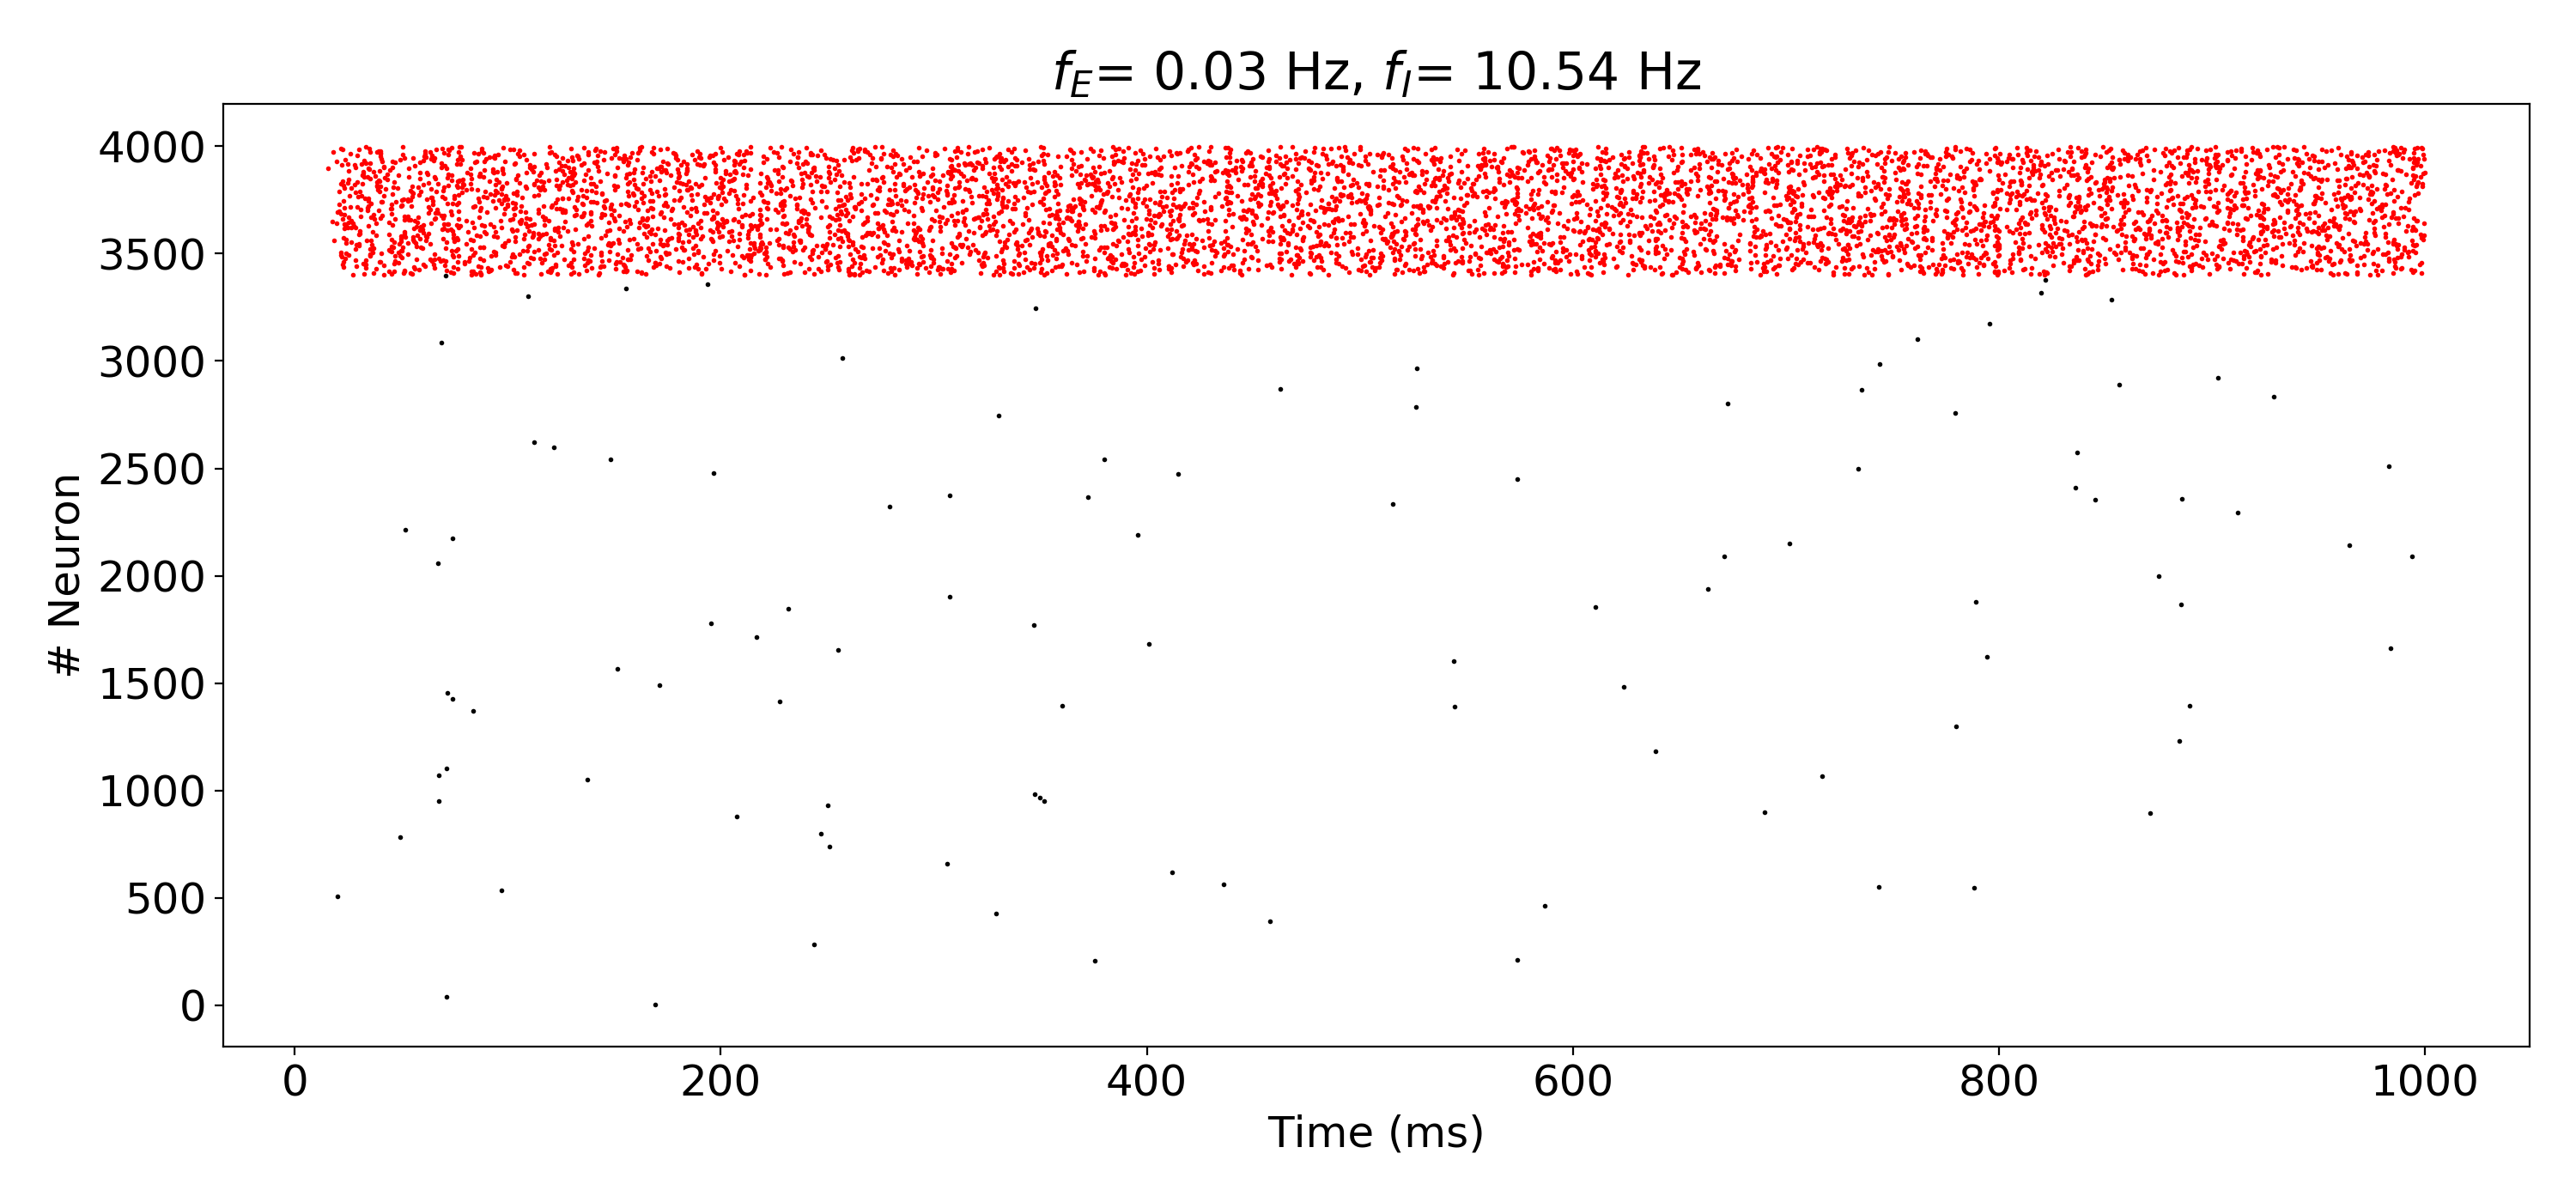
\includegraphics[width=1.0\textwidth]{figures/BKG_raster_plot.png}
\caption{\label{fig:BKG} Raster plot of network spiking activity when there is only background input as external stimulus. The red dots represent spikes from the inhibitory population and the black dots represent spikes from the excitatory population.}
\end{figure}
\FloatBarrier

\subsubsection{Dynamics of conditioning and extinction processes}

In Figure~\ref{fig:raster_COND_EXT}\textbf{A} we show the raster plot of spiking activity during the conditioning and extinction processes. The activities of subpopulations A and B, which represent fear and extinction neurons, respectively, are highlighted. After each presentation of $CS$ during the conditioning phase, there is an increase in the firing rate of $pop_A$. On the other hand, in the extinction phase, after the first presentations of $CS$ the $pop_A$ firing rate gradually decreases while the firing rate of $pop_B$  increases (Figure~\ref{fig:raster_COND_EXT}\textbf{B}). During these phases, the activity of the inhibitory neurons slightly fluctuated for each presentation of $CS$ as shown in Figure~\ref{fig:raster_COND_EXT}\textbf{C}.

\begin{figure}[!ht]
\centering
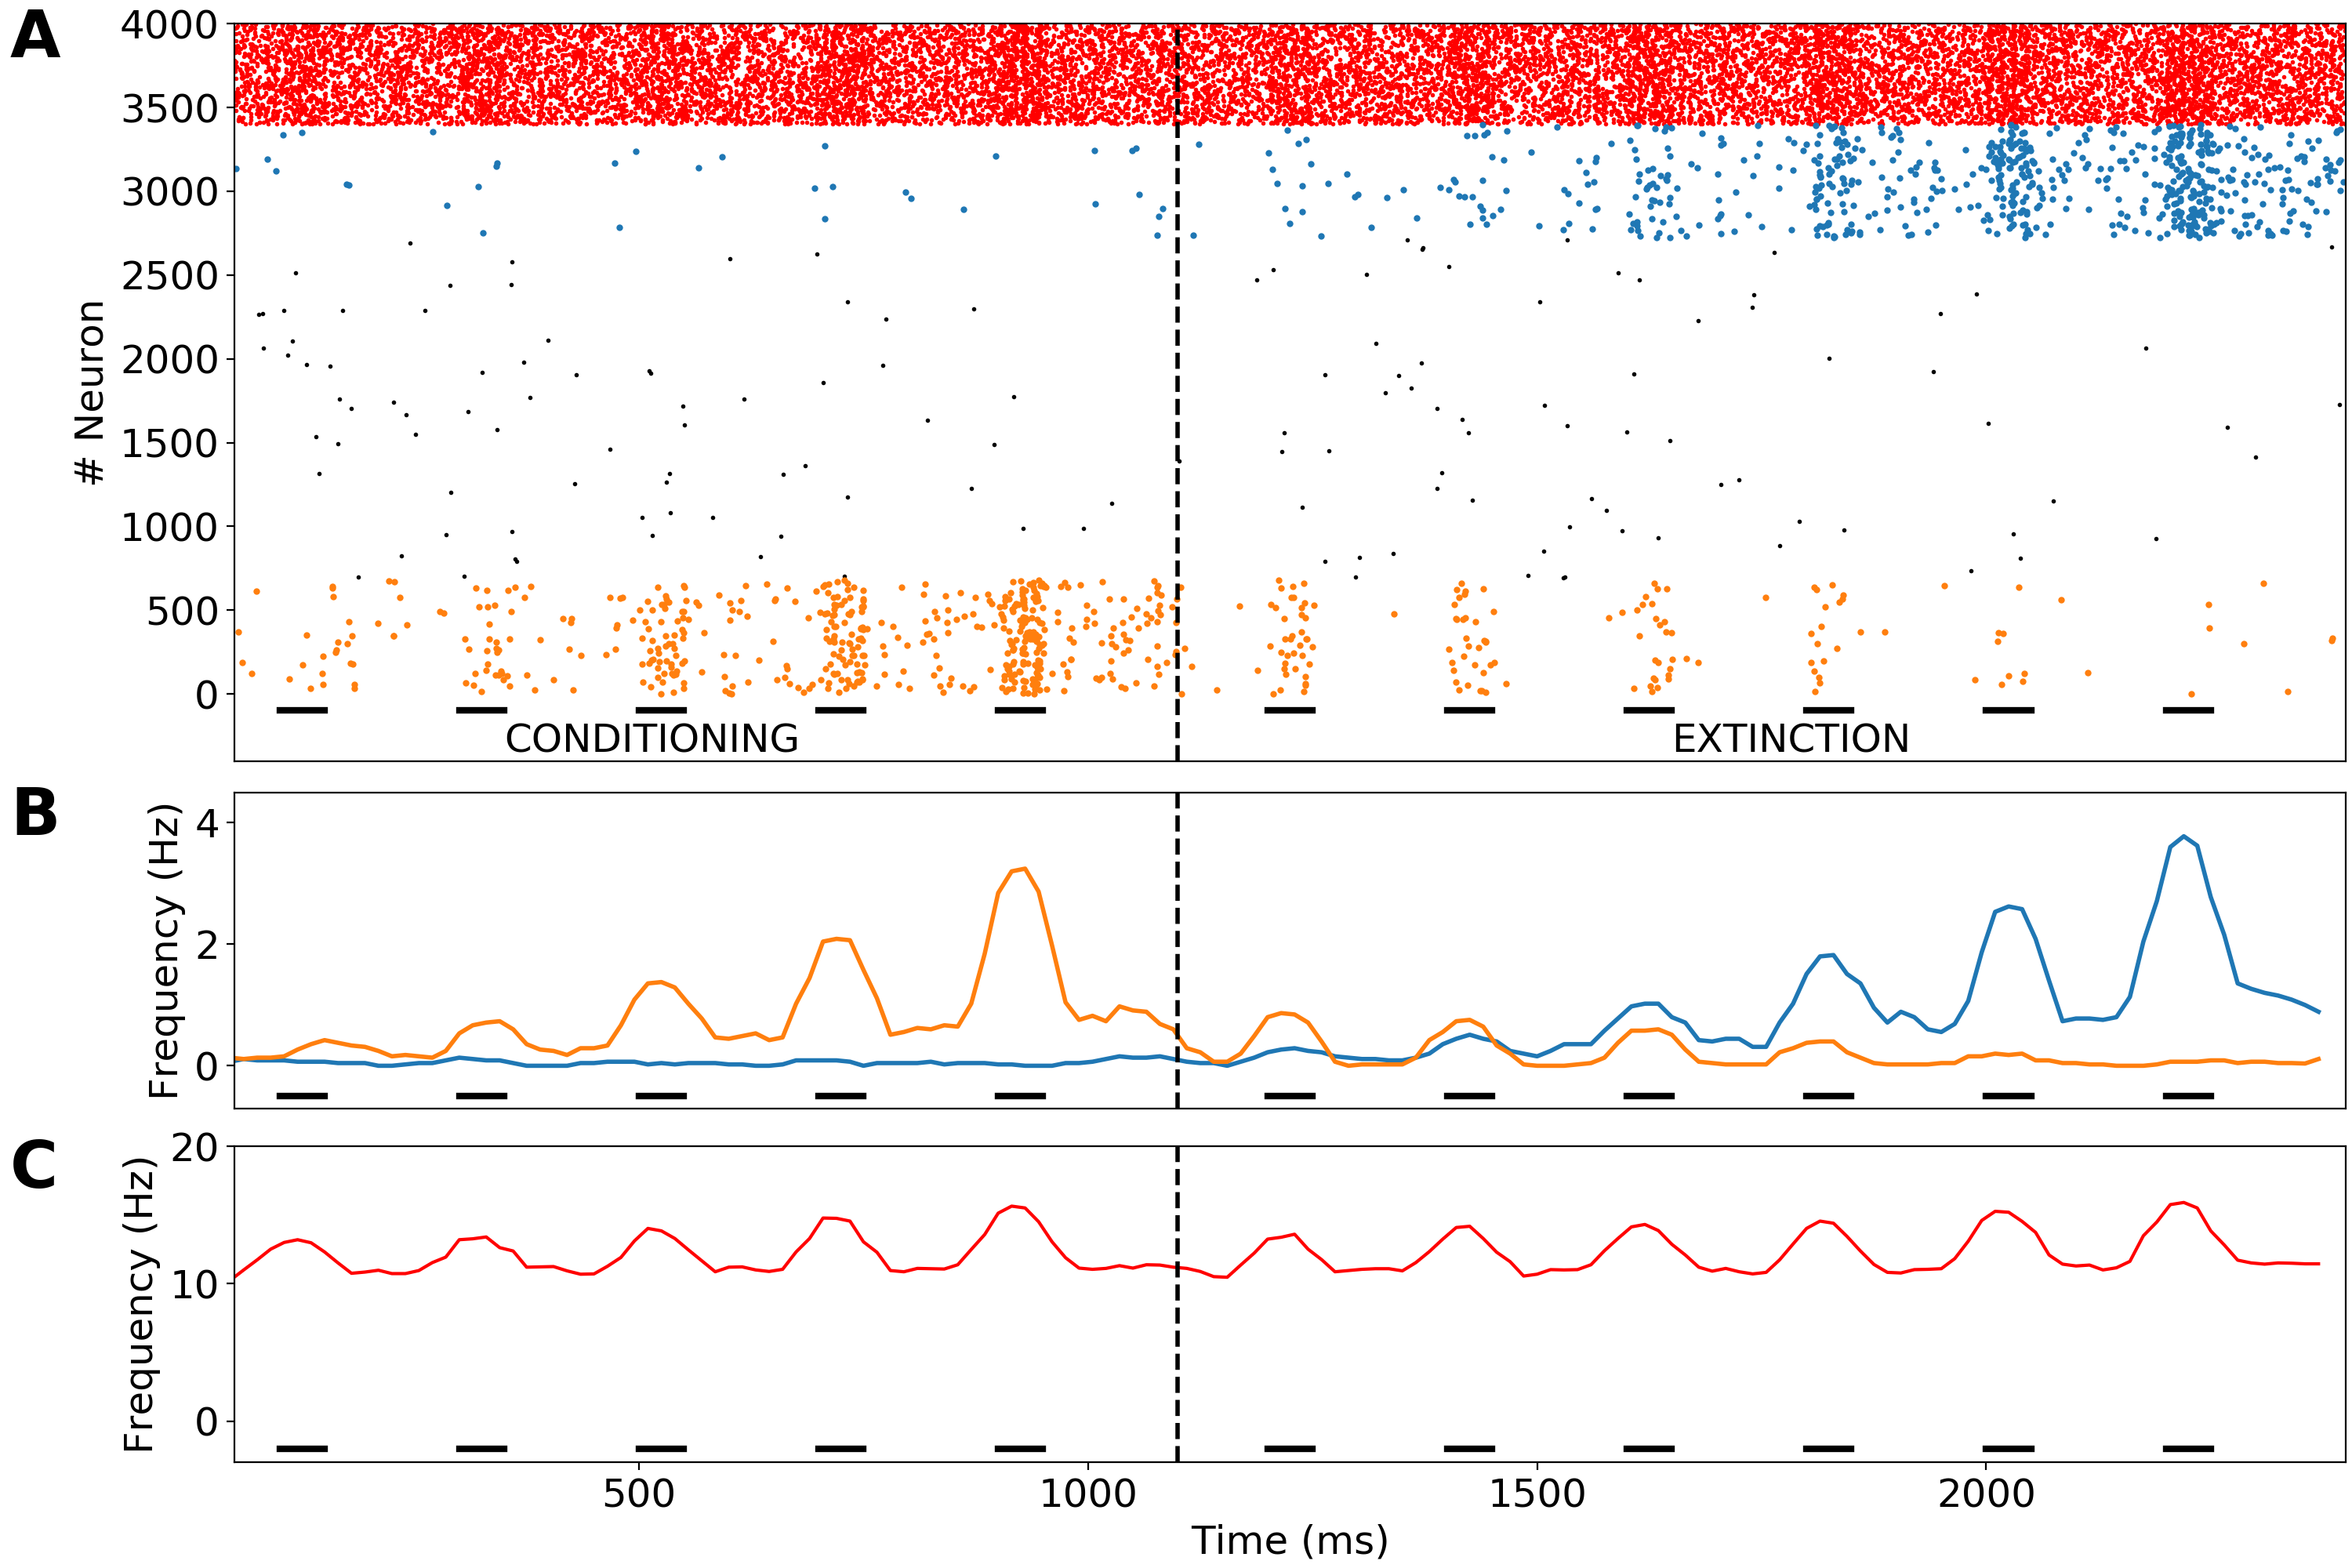
\includegraphics[width=1.0\textwidth]{figures/COND_EXT_raster.png}
\caption{\label{fig:raster_COND_EXT} Dynamics of the spiking network model of BA. This figure should be compared to Figures 5\textbf{A}-\textbf{C} of the reference paper. (\textbf{A}) Raster plot of simulated spiking network activity during the conditioning and extinction phases. The amber and cyan dots represent $pop_A$ and $pop_B$, respectively, while the red dots represent the inhibitory neuron population and the black dots represent the other excitatory neurons. (\textbf{B}) Firing rate per neuron of $pop_A$ and $pop_B$ (same colors as in \textbf{A}). (\textbf{C}) Firing rate per neuron of the inhibitory population. In (\textbf{B}) and (\textbf{C}) we used $\Delta t = 15$~ms. The loosely dashed horizontal lines symbolize the $CS$ presentations during the simulation and the vertical dashed line marks the transition from conditioning to extinction phase.}
\end{figure}
\FloatBarrier

In the caption of Figure 5 of the reference article, the authors explain that $pop_A$ and $pop_B$, each one, corresponds to 50\% of the total excitatory neurons. However, this is in disagreement with the methodology presented by them. In our study, we considered 20\% of the total excitatory neurons for each subpopulation as described in the original methodology and shown in Figure~\ref{fig:esquema_rede}.

We evaluated 30 simulations for the conditioning and extinction dynamics, and in all of them it was possible to verify the same scenario presented in Figure~\ref{fig:raster_COND_EXT}. In general, after each presentation of $CS$ there is an increase in synaptic weights associated with the $CTX$ applied followed by a decay when this $CTX$ is inactivated. Thus, the results relative to the average firing rates and synaptic weights (Figure~\ref{fig:weights_COND_EXT}) are consistent as expected from the synaptic plasticity rules applied (Equation~\ref{eq: plasticity}), and compatible with the original study.

\begin{figure}[!ht]
\centering
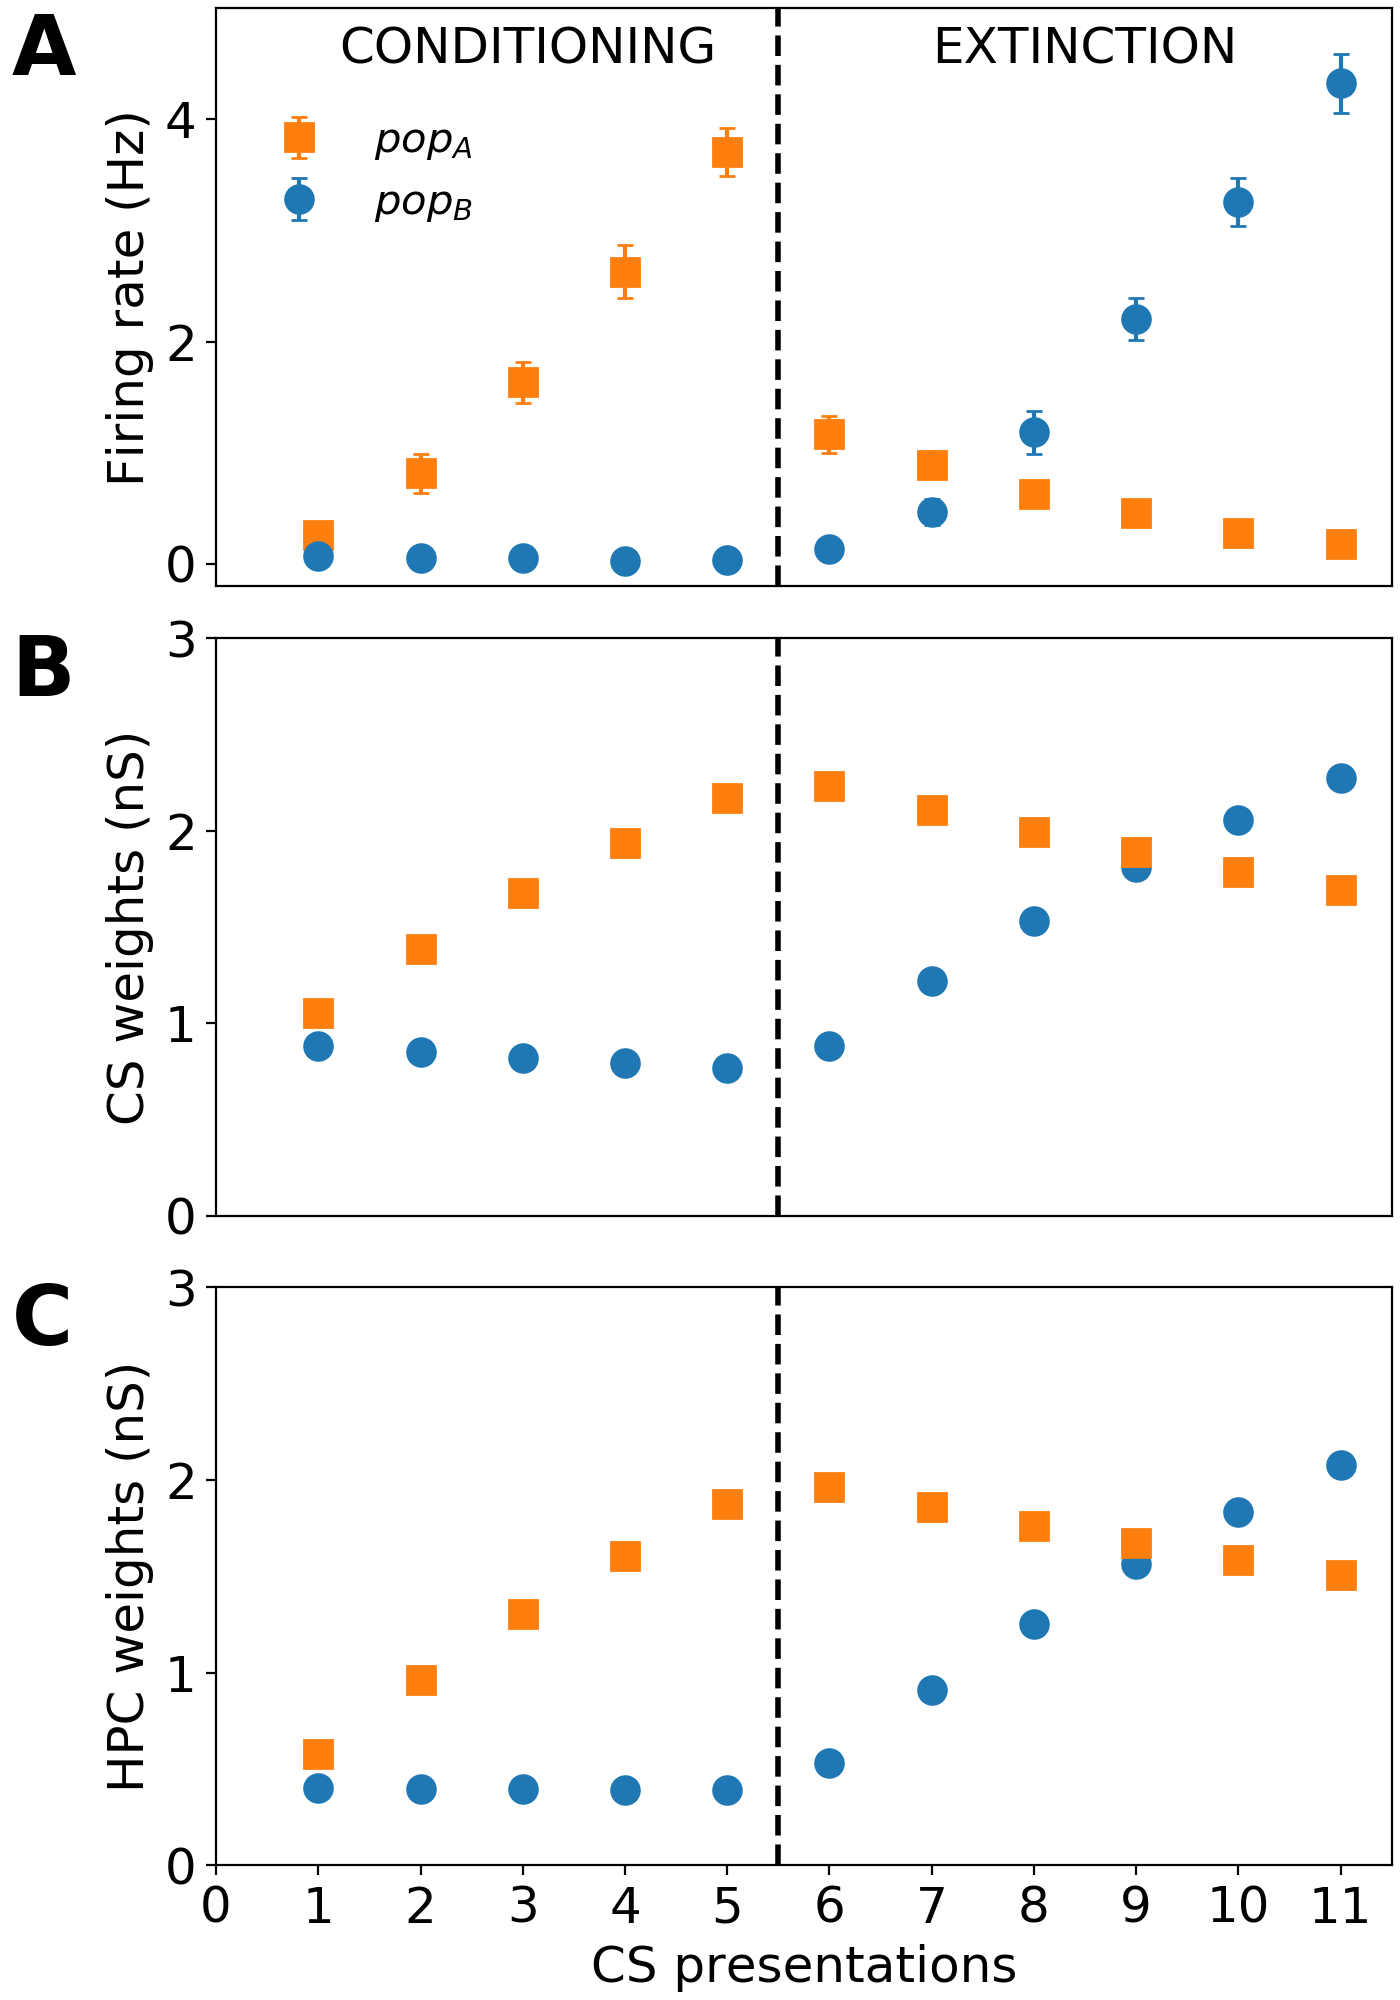
\includegraphics[width=8cm]{figures/COND_EXT_avarages.png}
\caption{\label{fig:weights_COND_EXT} Figure to be compared to Figures 5\textbf{E}-\textbf{J} of the reference paper. (\textbf{A}) Evolution of the firing rates of $pop_A$ and $pop_B$ neurons during fear conditioning (left) and extinction (right). Firing rates were evaluated over 30 simulations. (\textbf{B}) Evolution of synaptic weights of $CS$ inputs to $pop_A$ and $pop_B$ neurons during fear conditioning (left) and extinction (right). (\textbf{C}) Same as in (\textbf{B}) for the synaptic weights of $CTX$ inputs during $CS$ presentations. Here we chose to maintain the same acronym HPC used in the main reference, which refers to $CTX$.}
\end{figure}
\FloatBarrier

\subsubsection*{Fear renewal}
The results for these simulations are shown in Figures~\ref{fig:raster_RENEWAL}~and~\ref{fig:weights_RENEWAL}, and should be compared to Figures 7\textbf{A}-\textbf{C} and Figures 7\textbf{E}-\textbf{H} of the reference paper, respectively. In Figure~\ref{fig:raster_RENEWAL}\textbf{A} we show the spiking raster plot for the simulation, and in Figure~\ref{fig:raster_RENEWAL}\textbf{B-C} the activities of the excitatory and inhibitory populations, respectively. During the transition from the extinction to the renewal phase: i) the change of $CTX$ causes a sudden modification in the firing rates of $pop_A$ and $pop_B$ neurons (Figures~\ref{fig:raster_RENEWAL}\textbf{B}~and~\ref{fig:weights_RENEWAL}\textbf{A}); but ii) this effect barely influences the $CS$ and $CTX$ synaptic weights due to the synaptic plasticity rules (Figures~\ref{fig:weights_RENEWAL}\textbf{B}~and~\ref{fig:weights_RENEWAL}\textbf{C}).

In accordance with the reference article, the rapid change in the activity of subpopulations is a network phenomenon and not an effect of synaptic plasticity, although it plays an important role in the whole dynamics that precedes the renovation. Additionally, we observed a slight change in $CS$ and $CTX$ weights in the transition from extinction to renewal, which might be related to the difference between the time constants used in our replication and the original model (this could indicate that our $\tau_{h/c}$ is slightly faster) to simulate the synaptic plasticity.


\begin{figure}[!ht]
\centering
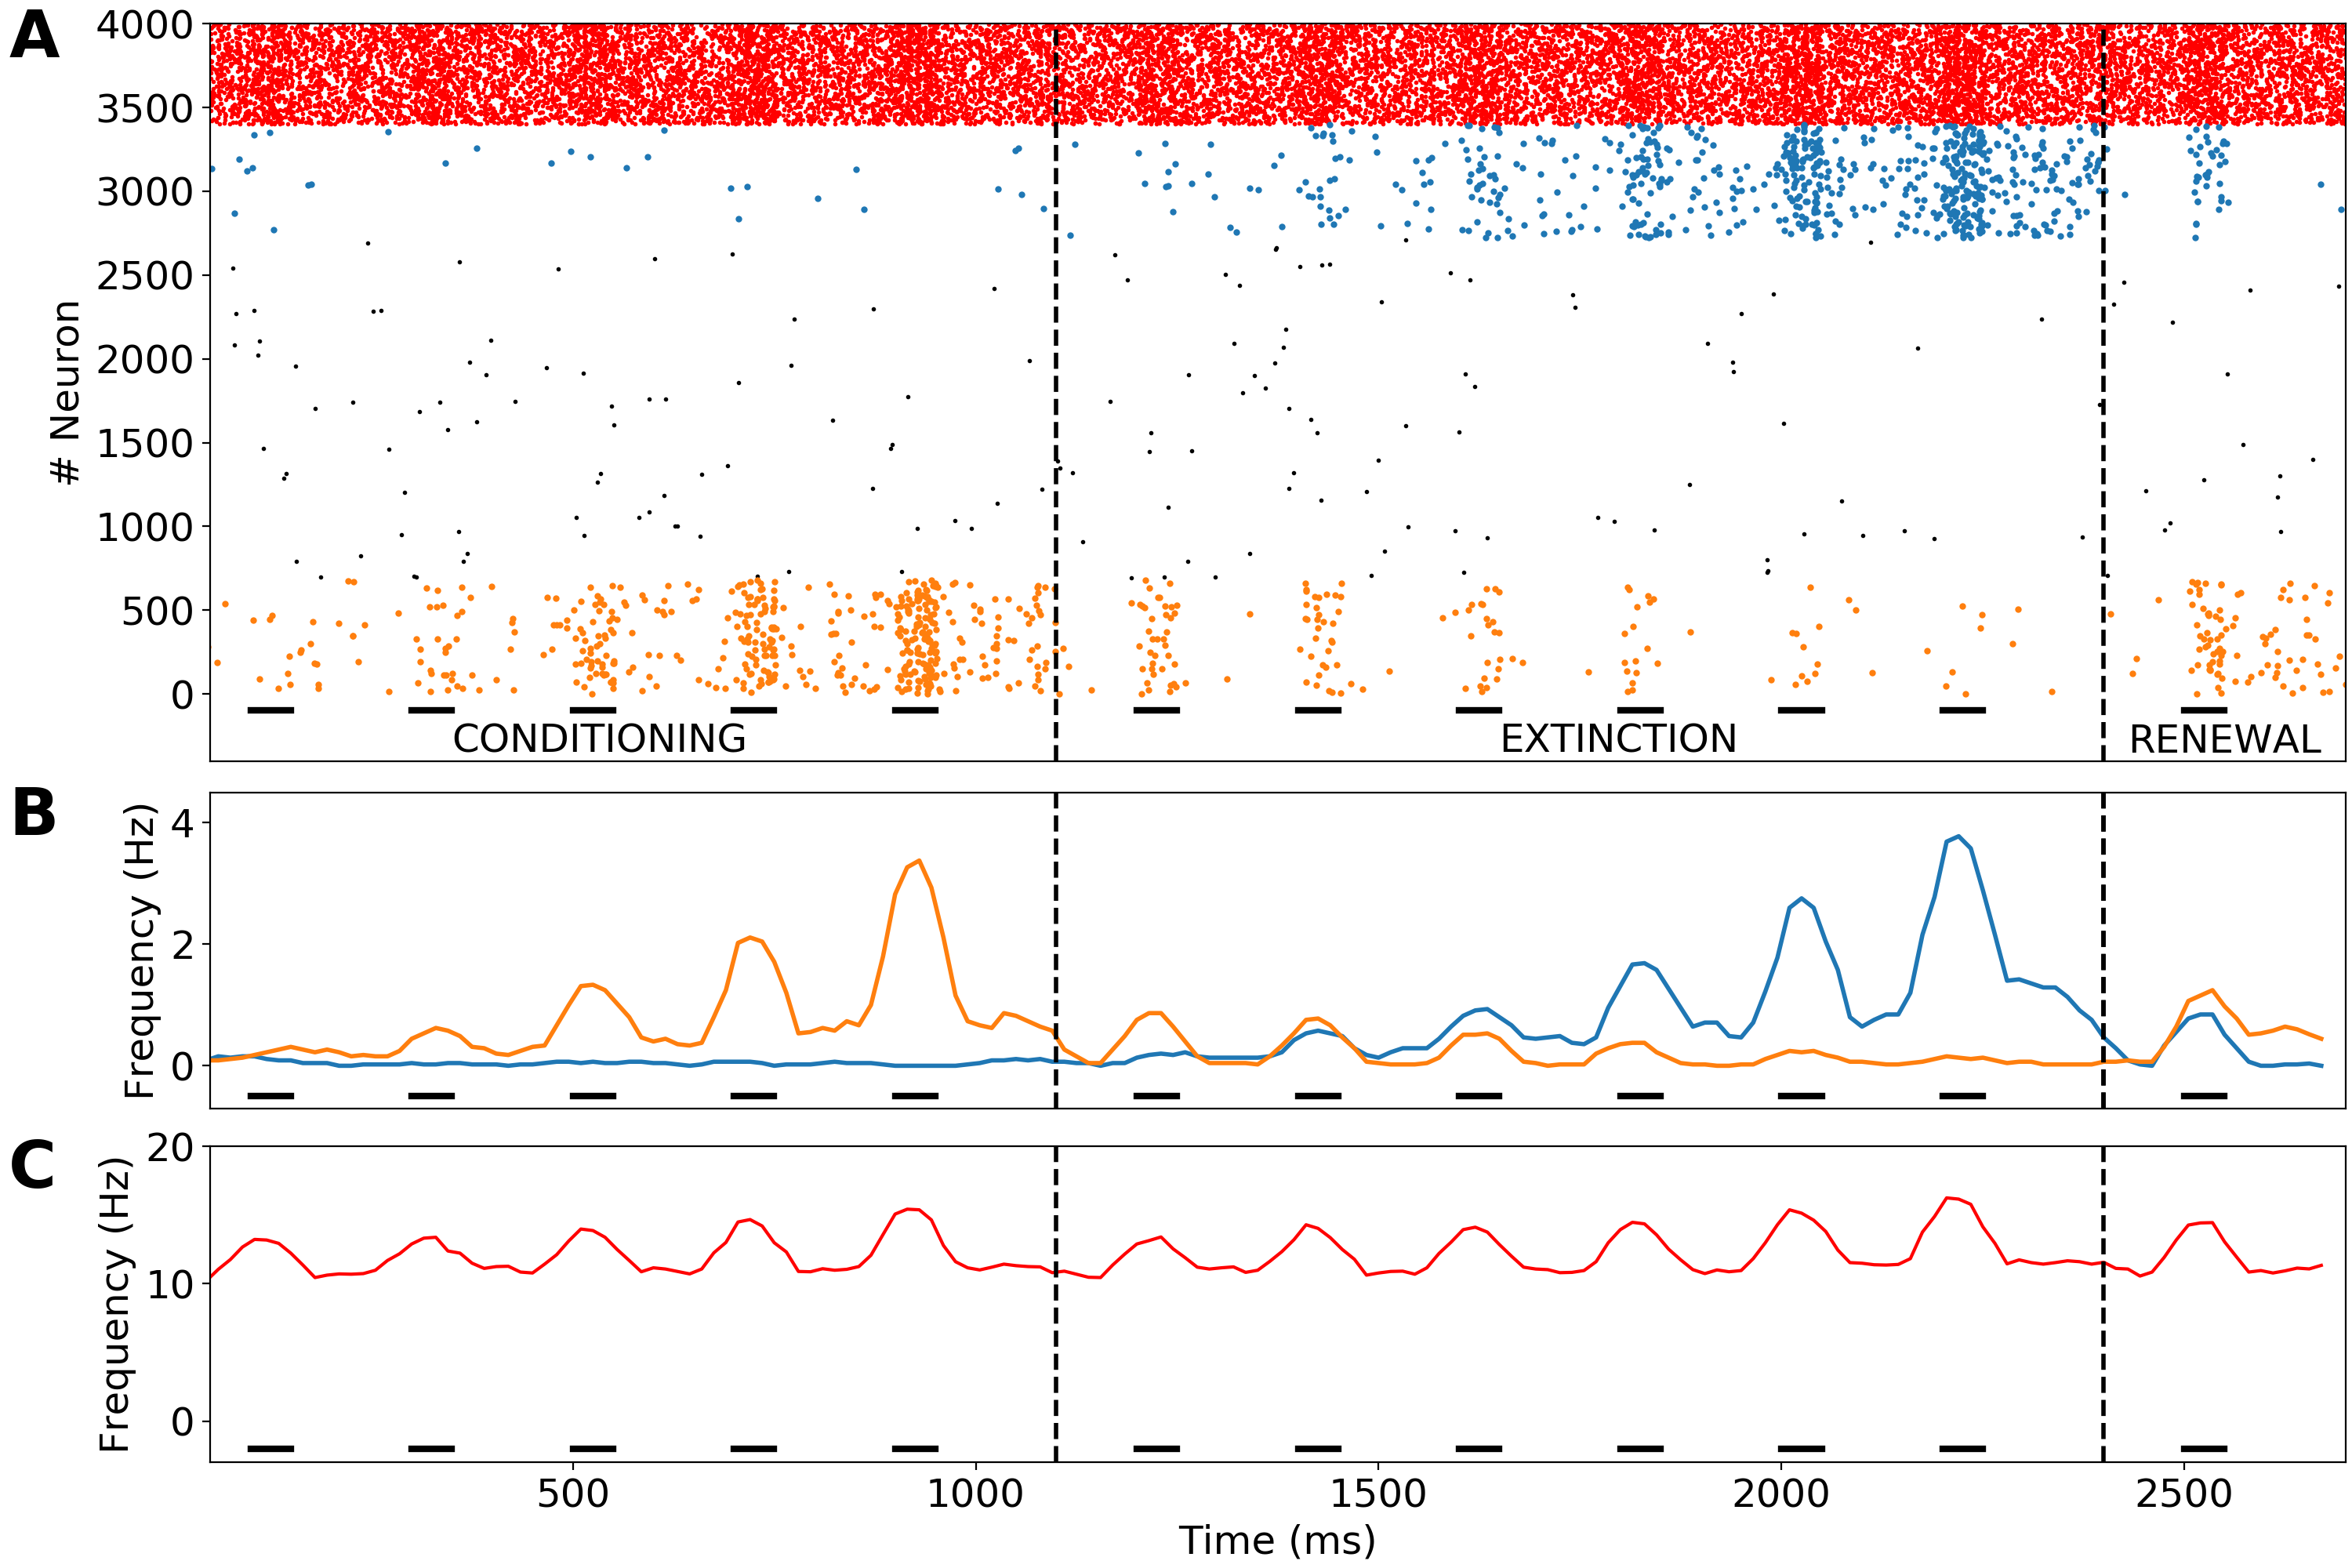
\includegraphics[width=1.0\textwidth]{figures/RENEWAL_raster.png}
\caption{\label{fig:raster_RENEWAL} ABA fear renewal. This scenario is equivalent to that shown in Figure~\ref{fig:raster_COND_EXT}, with the reactivation of $CTX_A$ and an additional presentation of CS. (\textbf{A}) Raster plot of spiking activity of fear (amber), extinction (cyan), inhibitory (red), and other excitatory (black) neurons. (\textbf{B}) Average firing rate of $pop_A$ and $pop_B$ neurons. (\textbf{C}) Average firing rate of the inhibitory neurons. Dashed horizontal lines symbolize the $CS$ presentations during the simulation and dashed vertical lines mark the transitions between conditioning and extinction and extinction and renewal. The exchange of $CTX$ after the extinction phase causes an instantaneous change in activity between $pop_A$ and $pop_B$ neurons. In (\textbf{B}) and (\textbf{C}) we used $\Delta t = 15$~ms.}
\end{figure}
\FloatBarrier

\begin{figure}[!ht]
\centering
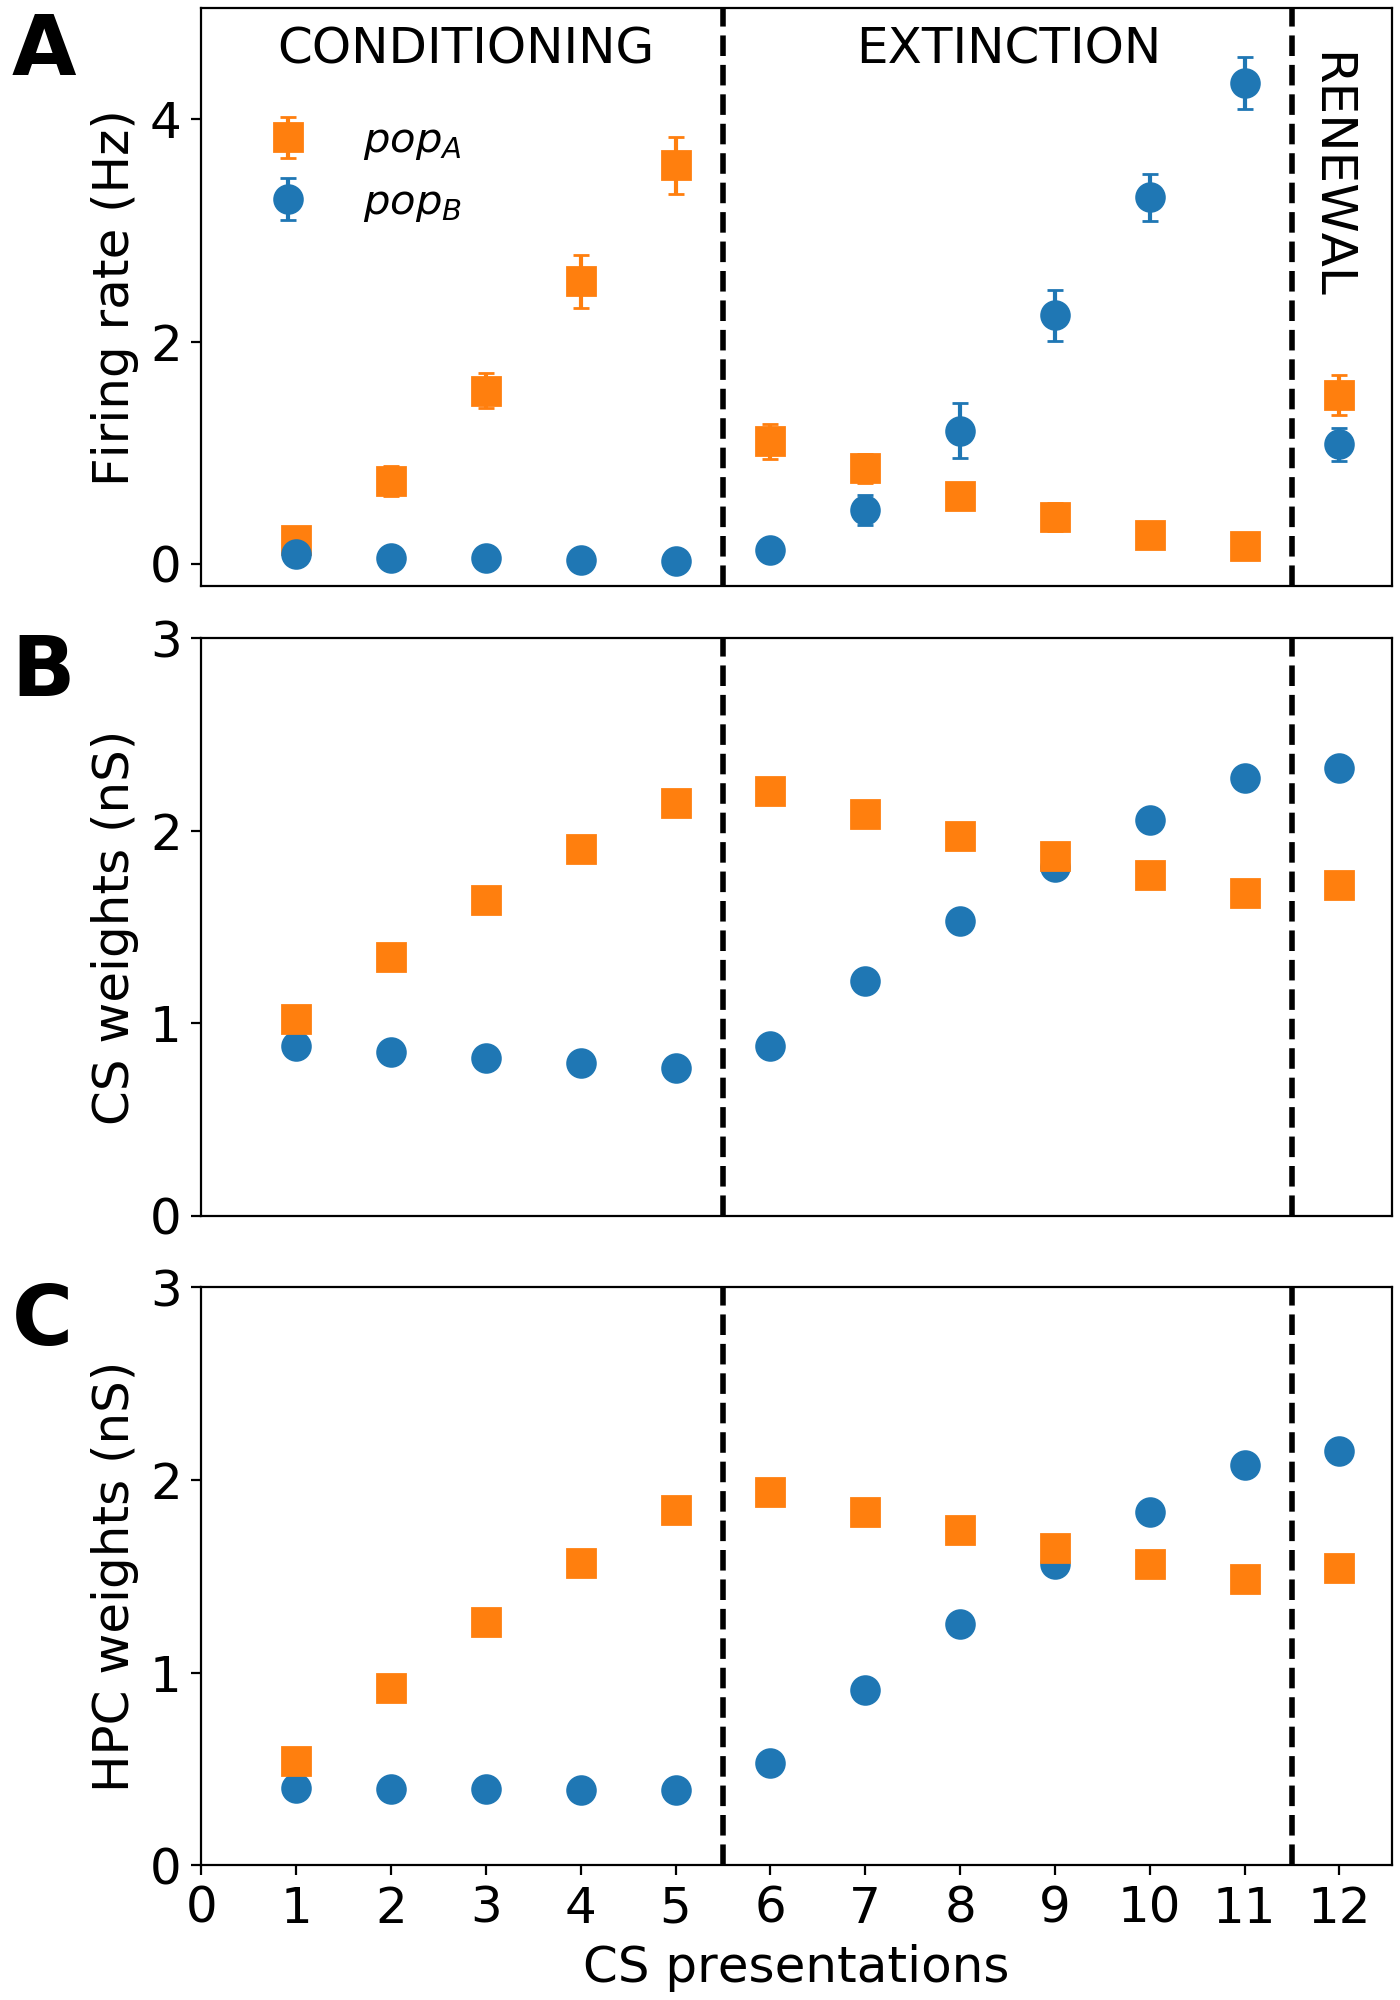
\includegraphics[width=8cm]{figures/RENEWAL_avarages.png}
\caption{\label{fig:weights_RENEWAL} (\textbf{A}) Average firing rates of $pop_A$ and $pop_B$ neurons during conditioning, extinction and renewal. Averages were performed over 30 simulations of ABA renewal. (\textbf{B}) Synaptic weights of $CS$ inputs to $pop_A$ and $pop_B$ neurons. (\textbf{C}) Synaptic weights of $CTX$ inputs during $CS$ presentations. Here we chose to maintain the same acronym HPC used in the reference article that refers to $CTX$. During renewal, the synaptic weights undergo slight changes because of the synaptic plasticity rule applied. Despite a decline in the synaptic weights of $pop_A$ at the end of the extinction phase, these weights still have higher values than at the beginning of the conditioning phase, thus when reactivating the $CTX_A$, the firing rate for $pop_A$ increases sharply. Note that in Figure 7F of the original article the colors used to indicated the populations are inverted.}
\end{figure}
\FloatBarrier

\subsubsection*{High connectivity introduces gamma oscillations}

In the corresponding section of the reference article, the connection probability $p_{II}$ (defined here in Table~\ref{tab: probability connection}) was increased to the experimentally reported value of $0.5$~\cite{woodruff2007networks} to study the effect of this high connectivity on the behavior of the spiking network model. The authors reported that this change in the network did not affect the qualitative behavior of the model but a new aspect emerged in the dynamics: gamma oscillations in the network firing rate.

With a careful inspection of Figure 8A of the main reference, we noted that the authors studied this phenomenon only for the conditioning phase and, to obtain a similar result, we increase the amount of $CS$ presentations to 10 (this result is dependent on the number of $CS$ presentations). The results for this procedure are shown in Figure~\ref{fig:gamma}.

\begin{figure}[!ht]
\centering
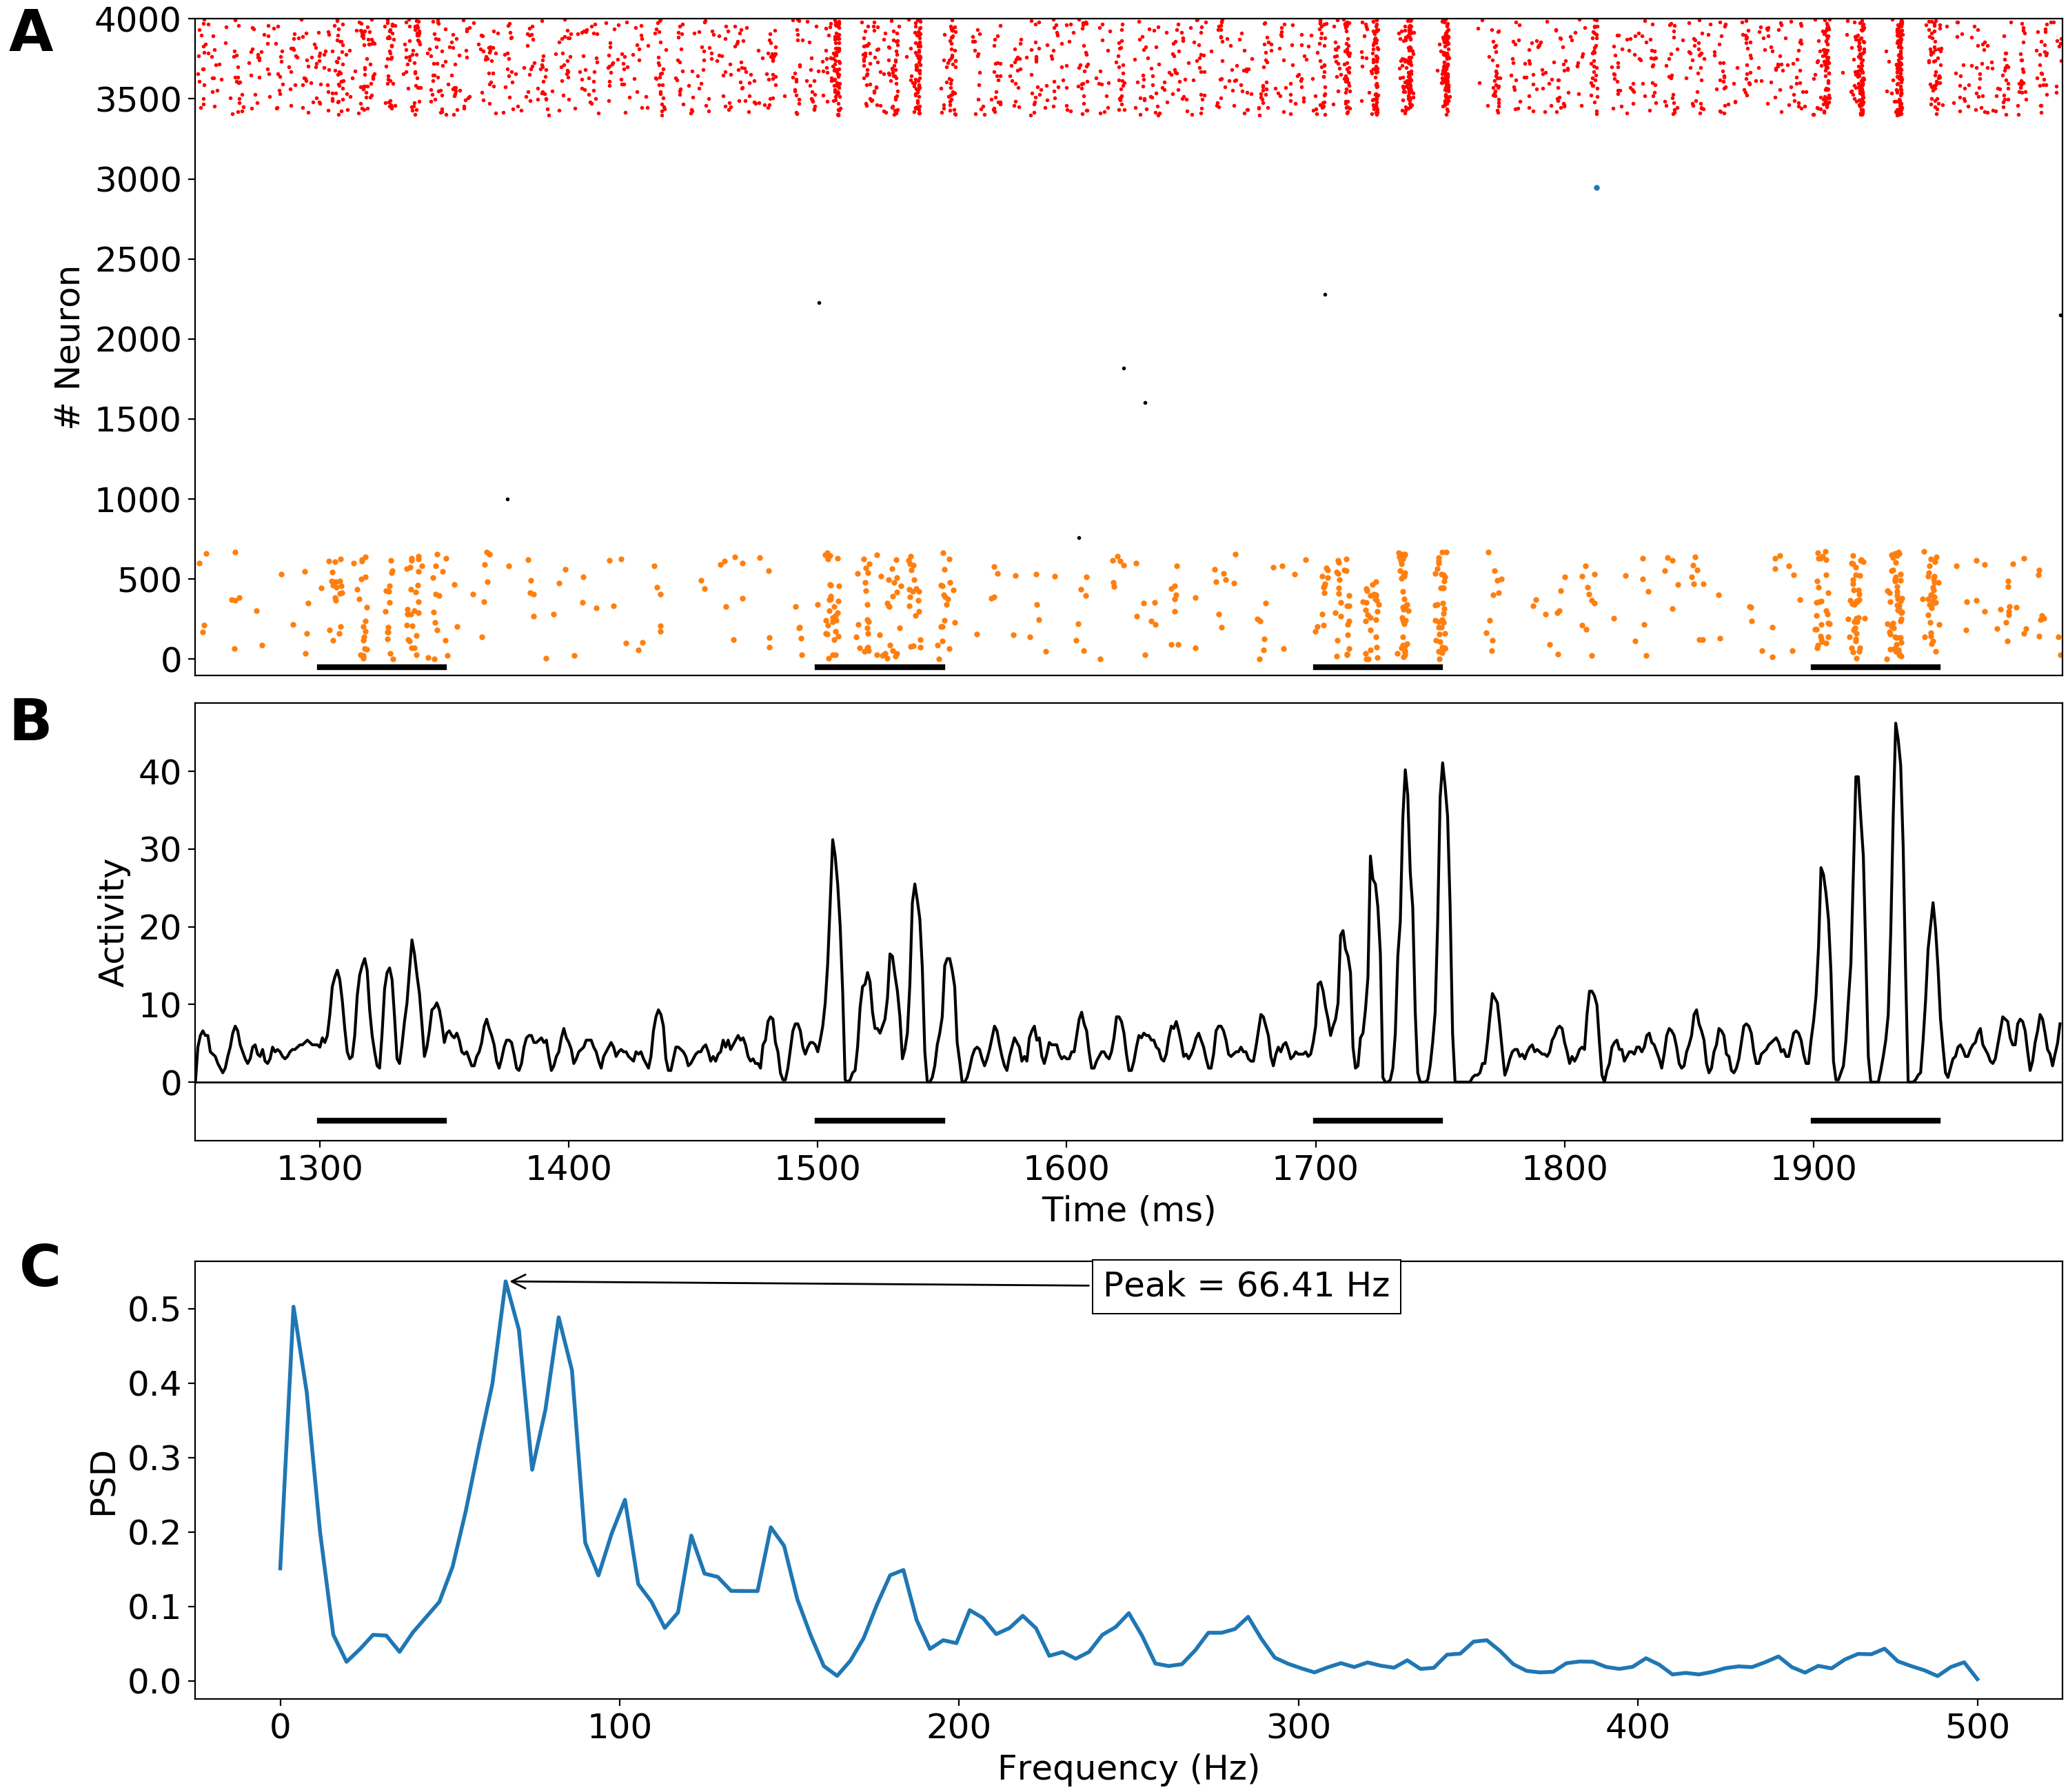
\includegraphics[width=1.0\textwidth]{figures/gamma_oscillations.png}
\caption{\label{fig:gamma} Gamma oscillations for high network connectivity. (\textbf{A}) Raster plot of spiking activity for the last 4 presentations of $CS$ during the conditioning phase. Amber dots represent the fear neurons, red dots the inhibitory neurons, and black dots the other excitatory neurons. (\textbf{B}) Histogram (smoothed) of population activity. During each presentation of $CS$ (horizontal black lines), it is possible to notice signatures of gamma oscillations. (\textbf{C}) Power spectrum density of the time series in (\textbf{B}). The peak at 66.41 Hz (in the gamma band) is indicated by an arrow.}
\end{figure}
\FloatBarrier

In Figure~\ref{fig:gamma}A, we show a raster plot of the spiking activity for the last four $CS$ presentations. At each presentation the neurons fire in a more synchronous fashion as can be seen in Figure~\ref{fig:gamma}B. The $PSD$ of this synchronous activity is shown in Figure~\ref{fig:gamma}C and it displays a peak at 66.41~Hz, within the gamma oscillation range (30-80~Hz). Thus, through our approximation, we obtained a similar result to that observed in Figure 8A of the original work.

Further, the authors investigated how the network properties impact the overall synchrony. To illustrate the meaning of the synchrony index used in this replication, in Figure~\ref{fig:examples_synchrony} we show time series of the synchrony index for three different types of activity of the inhibitory population (obtained with different values of $p_{II}$). As gamma oscillations emerge, the synchrony index increases. In particular, we show that the oscillatory power of the network is positively correlated with the synchrony index. Specifically for this network the characteristic oscillations are always within the gamma band. We will assume that a synchrony index greater than 4.5 characterizes the presence of gamma oscillations. %gamma oscillations in the network occur when the synchrony is greater than 4.5.

\begin{figure}[!ht]
\centering
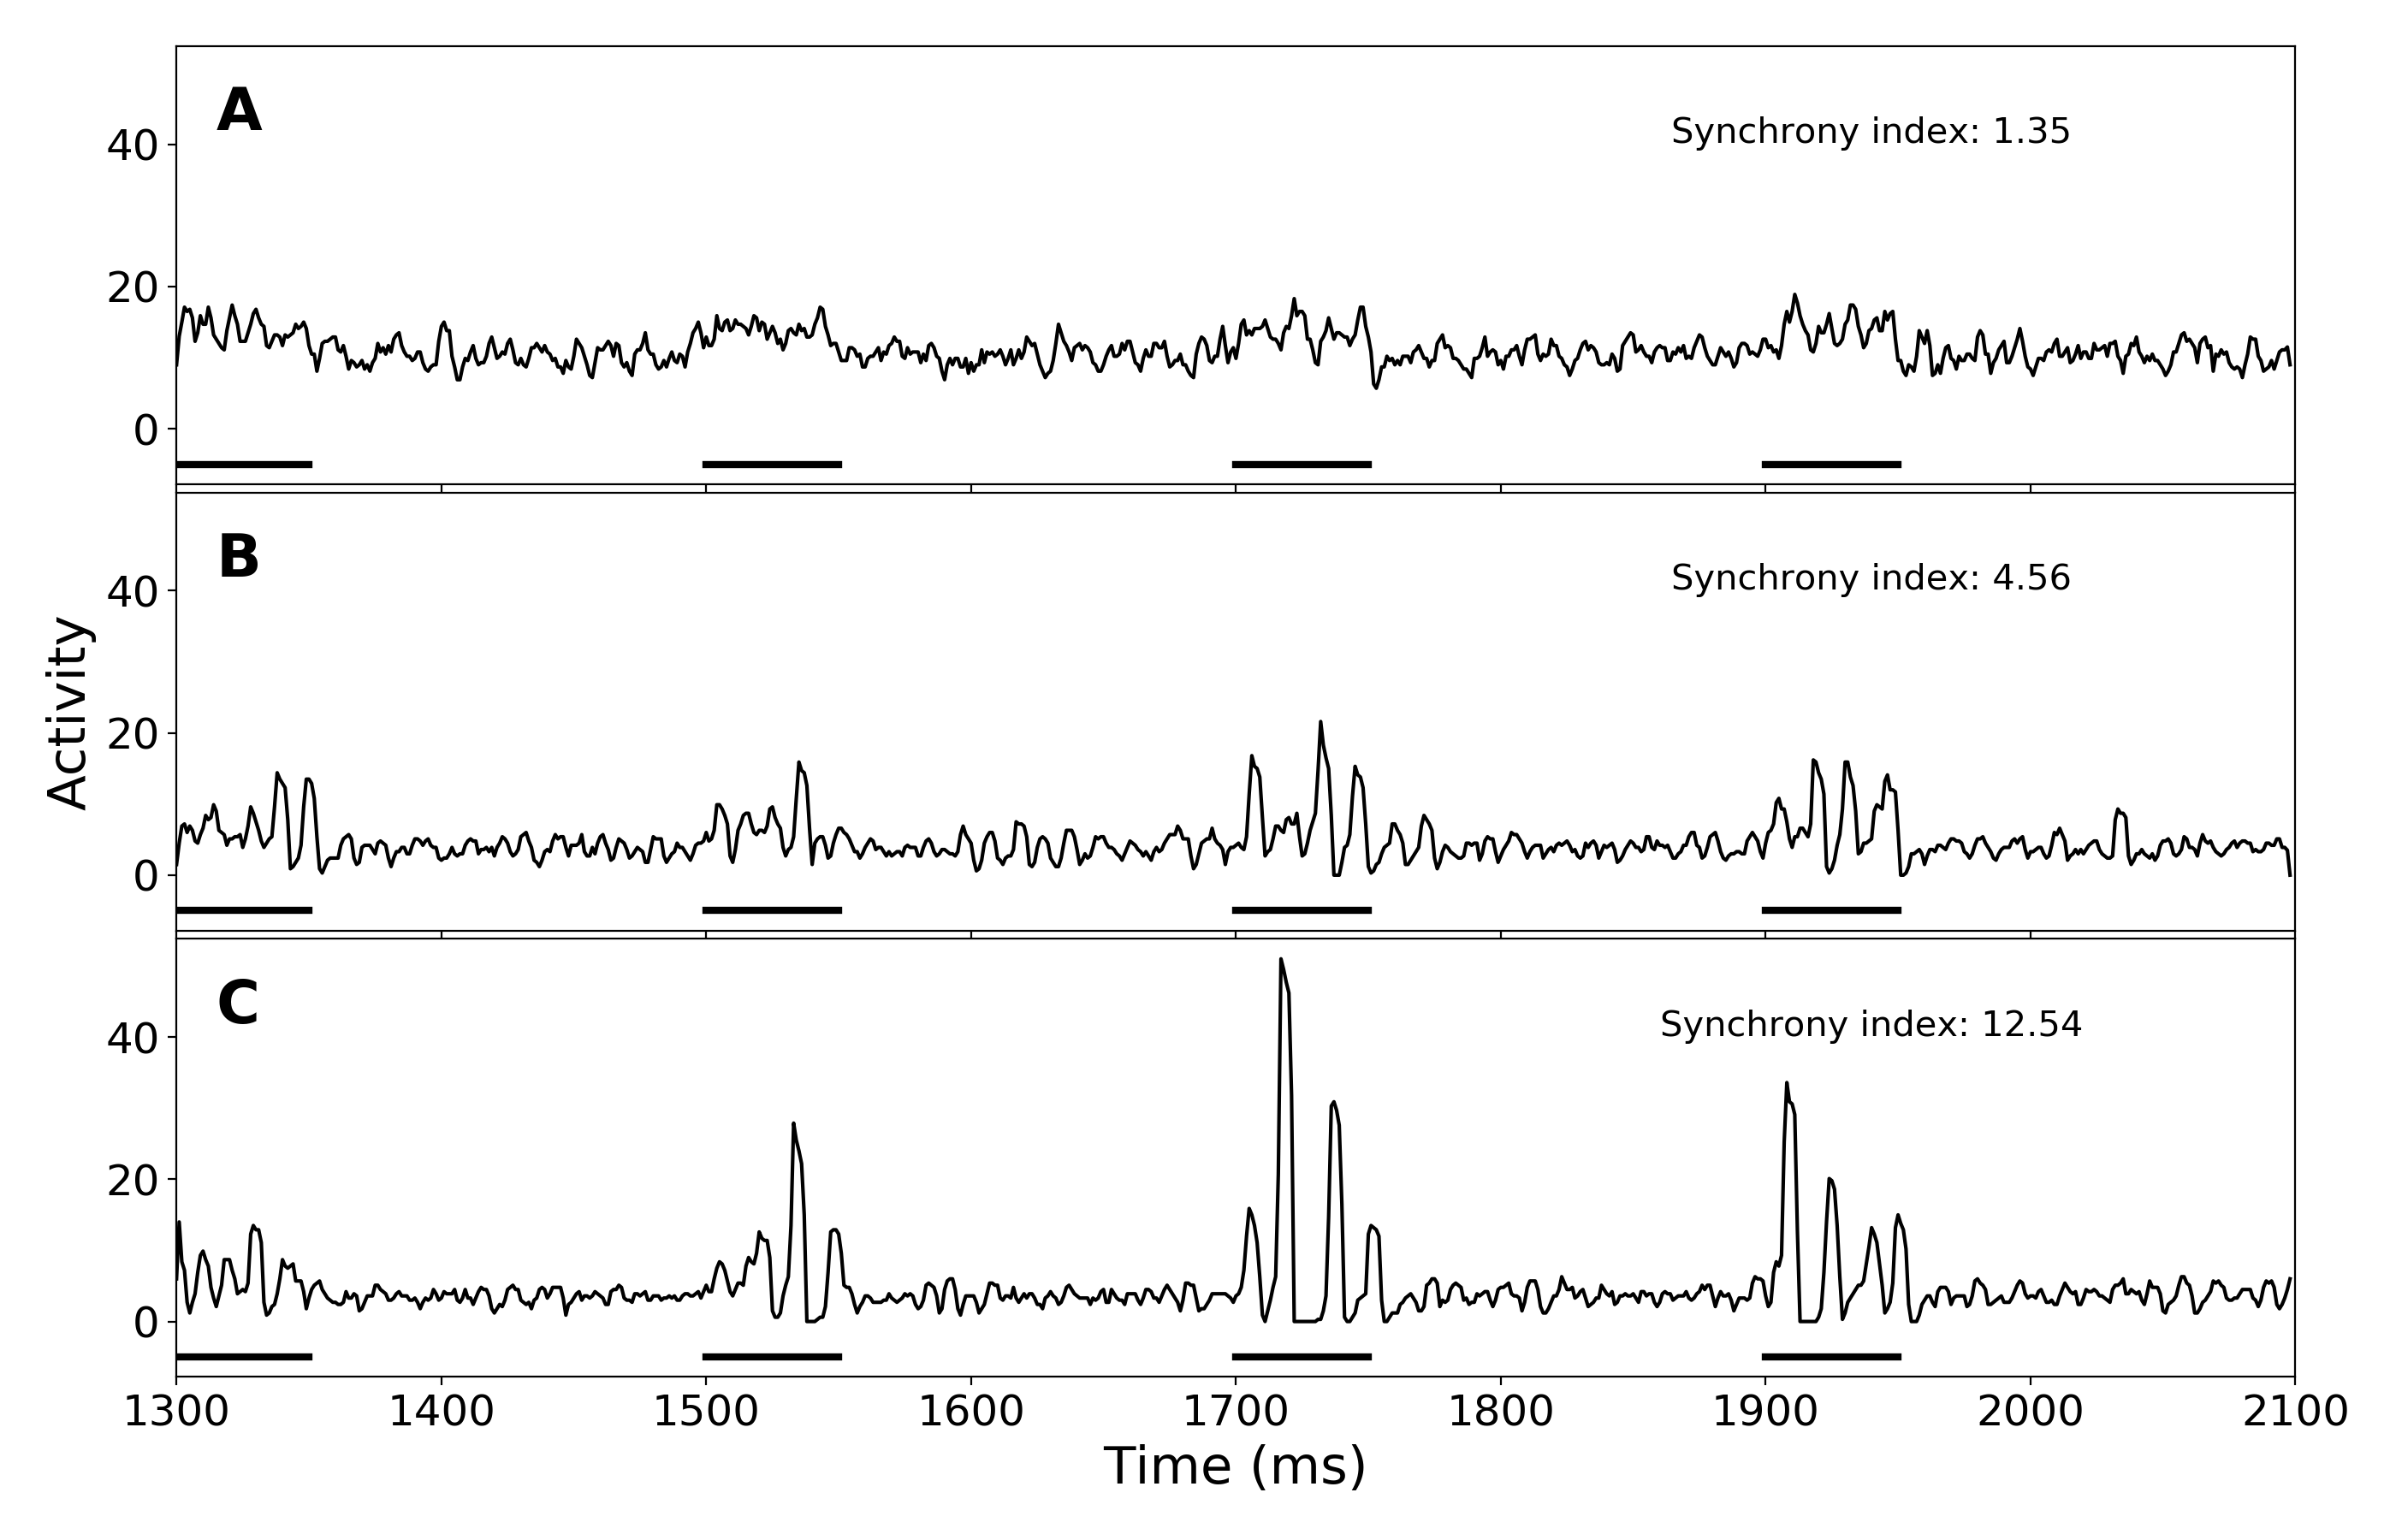
\includegraphics[width=1.0\textwidth]{figures/examples_synchrony_index.png}
\caption{\label{fig:examples_synchrony} Synchrony index and gamma oscillations. (\textbf{A}) Non-synchronized case. (\textbf{B}) Synchronized case with emergence of gamma oscillations. (\textbf{C}) Synchronized case with strong gamma oscillations. The synchronization index shown above each plot was calculated using the activity of the inhibitory population obtained with a histogram of bin size $\Delta t =1$ ms, delay distributed uniformly between $[1.0-2.0]$ for an inhibitory synaptic weight of 2 nS. The times series were generated with three different values of connection probability among inhibitory neurons: (\textbf{A}) $p_{II} = 0.1$, (\textbf{B}) $p_{II} = 0.6$, and (\textbf{C}) $p_{II} = 0.7$.}
\end{figure}
\FloatBarrier


To explore mechanisms operating in BA that could dampen gamma oscillations, the authors of the original text investigated the measure of synchrony as a function of connectivity, synaptic weights and delays between inhibitory neurons. The $p_{II}$ connectivity was analyzed from $0.1$ to $0.9$, at $0.1$ intervals; synaptic weights $w_{II}$ were set to $1$, $2$ or $3$ nS; and delays were divided in two groups: ``higher'', uniformly distributed between $[1.0-2.0]$~ms, and ``lower'', uniformly distributed between $[0.2-1.0]$ ms. 

Figure~\ref{fig:synchrony} shows the synchrony index for simulations with all possible combinations of these three groups of parameters. Gamma oscillations are not present (regions bellow the purple dashed line in Figure~\ref{fig:synchrony}) for both delay scenarios (``higher'' and ``lower'') when one of the following conditions is true: (i) $p_{II}$ lower than $0.4$, or (ii) $w_{II} = 1$ nS independently of $p_{II}$. For delay type ``lower'', there is a reduction of oscillations in all situations, which is compatible with the reference article. Thus, changes in the inhibitory structure of the network are essential to obtain gamma oscillations in neuronal activity.

\begin{figure}[!ht]
\centering
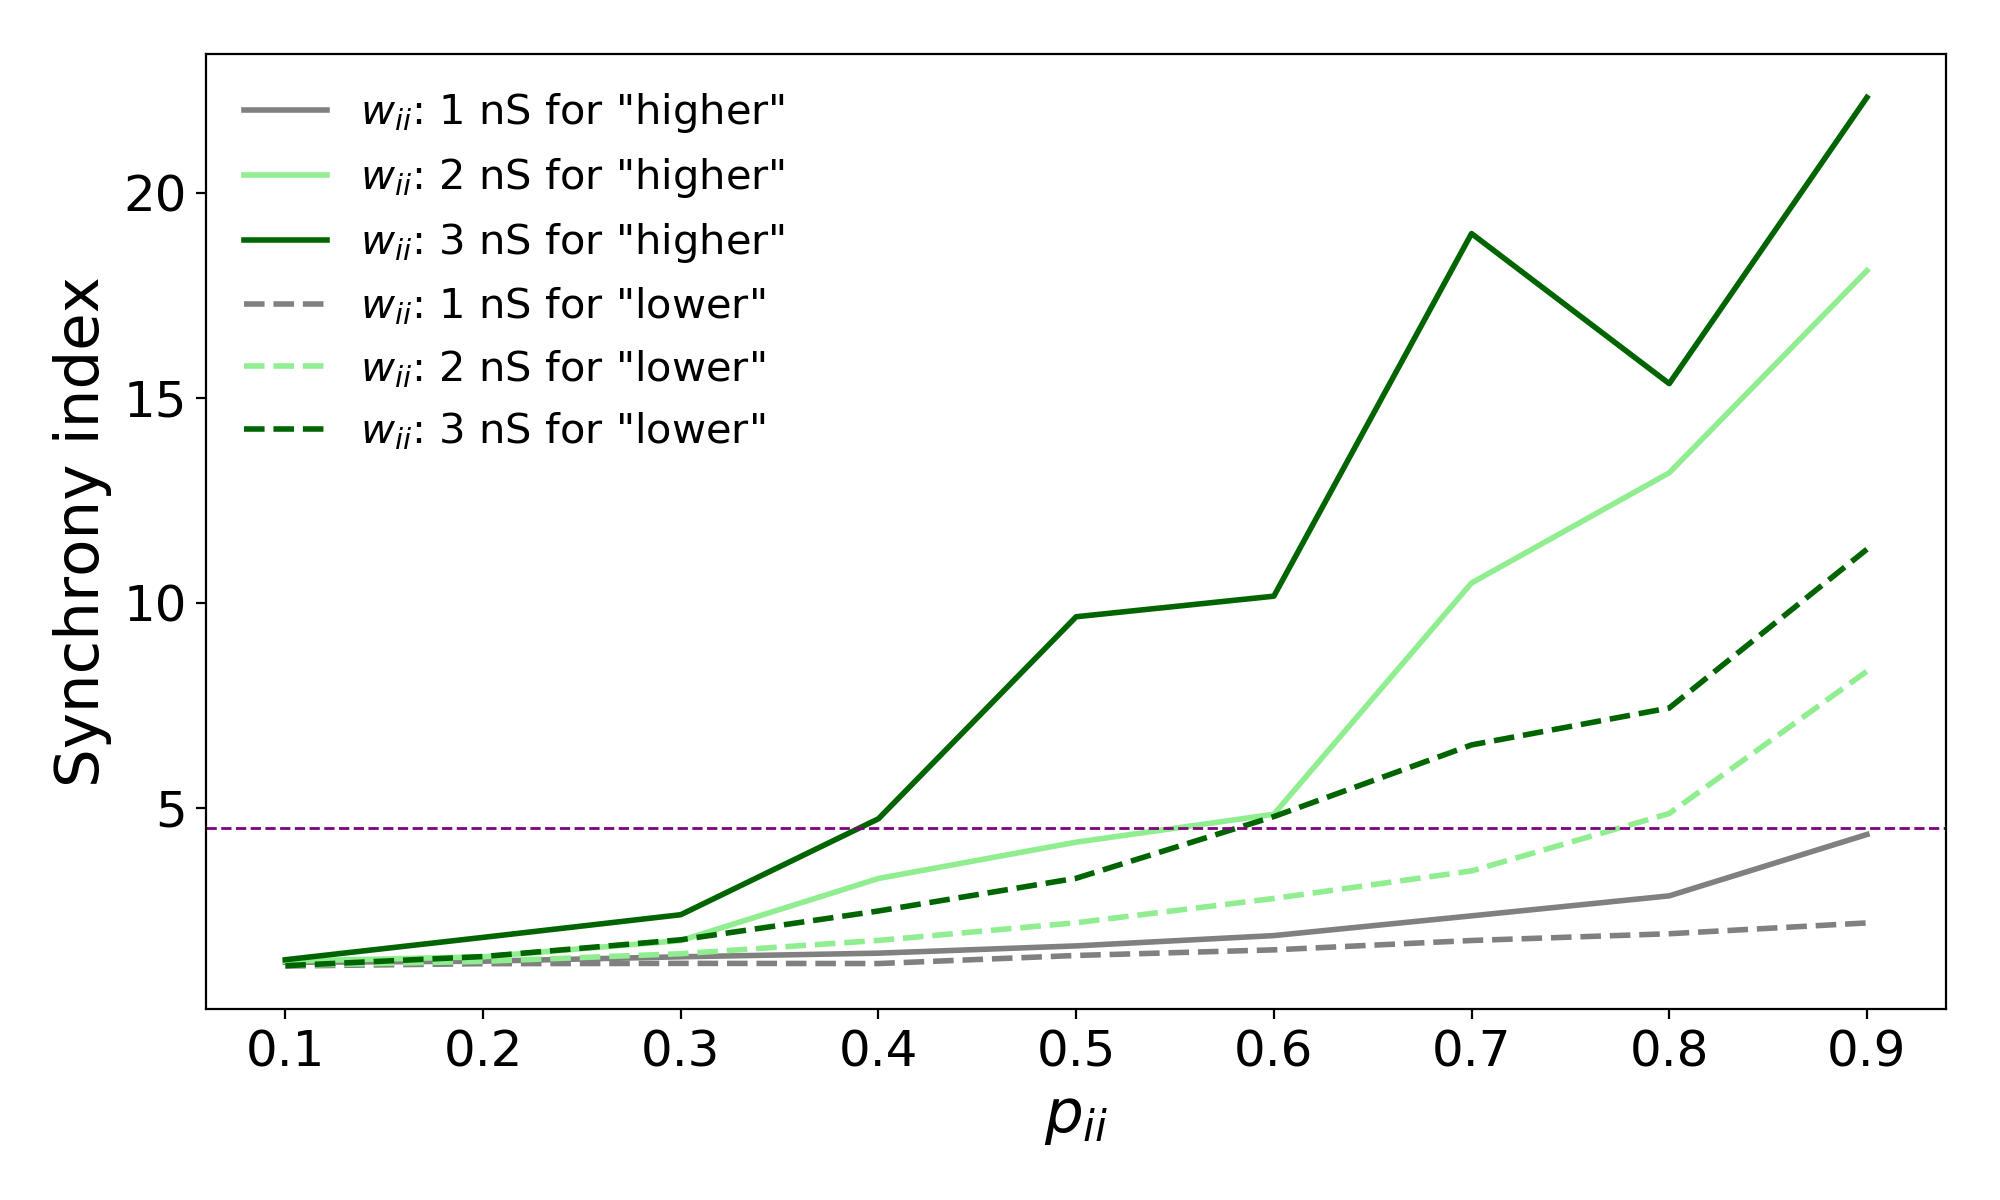
\includegraphics[width=1.0\textwidth]{figures/synchrony_index.png}
\caption{\label{fig:synchrony} Effects of connectivity, synaptic weights and delays of the inhibitory population on synchronization. The synchrony index used was the Fano factor calculated on the histogram of inhibitory spikes during the presentation of the last four $CS$ during the conditioning phase. The combinations between synaptic weights and delays are indicated by different colors (gray, light green and dark green) and line types (continuous or dashed) as indicated on the left-hand top corner. The purple dashed line indicates the threshold value 4.5 above which the synchrony index indicates gamma oscillations according to our definition.}
\end{figure}
\FloatBarrier


\subsubsection{Blockage of inhibition}

Inhibition plays an important role in controlling the firing rate of the network as can be seen in Figure~\ref{fig:raster_COND_EXT}A, in which the firing rate of excitatory neurons not belonging to subpopulations A and B (black dots) remains close to zero even with presentations of $CS$. Based on this, we performed two additional sets of simulations where we deactivated first $50\%$ and then $90\%$ of inhibitory neurons during the extinction phase.

\begin{figure}[!ht]
\centering
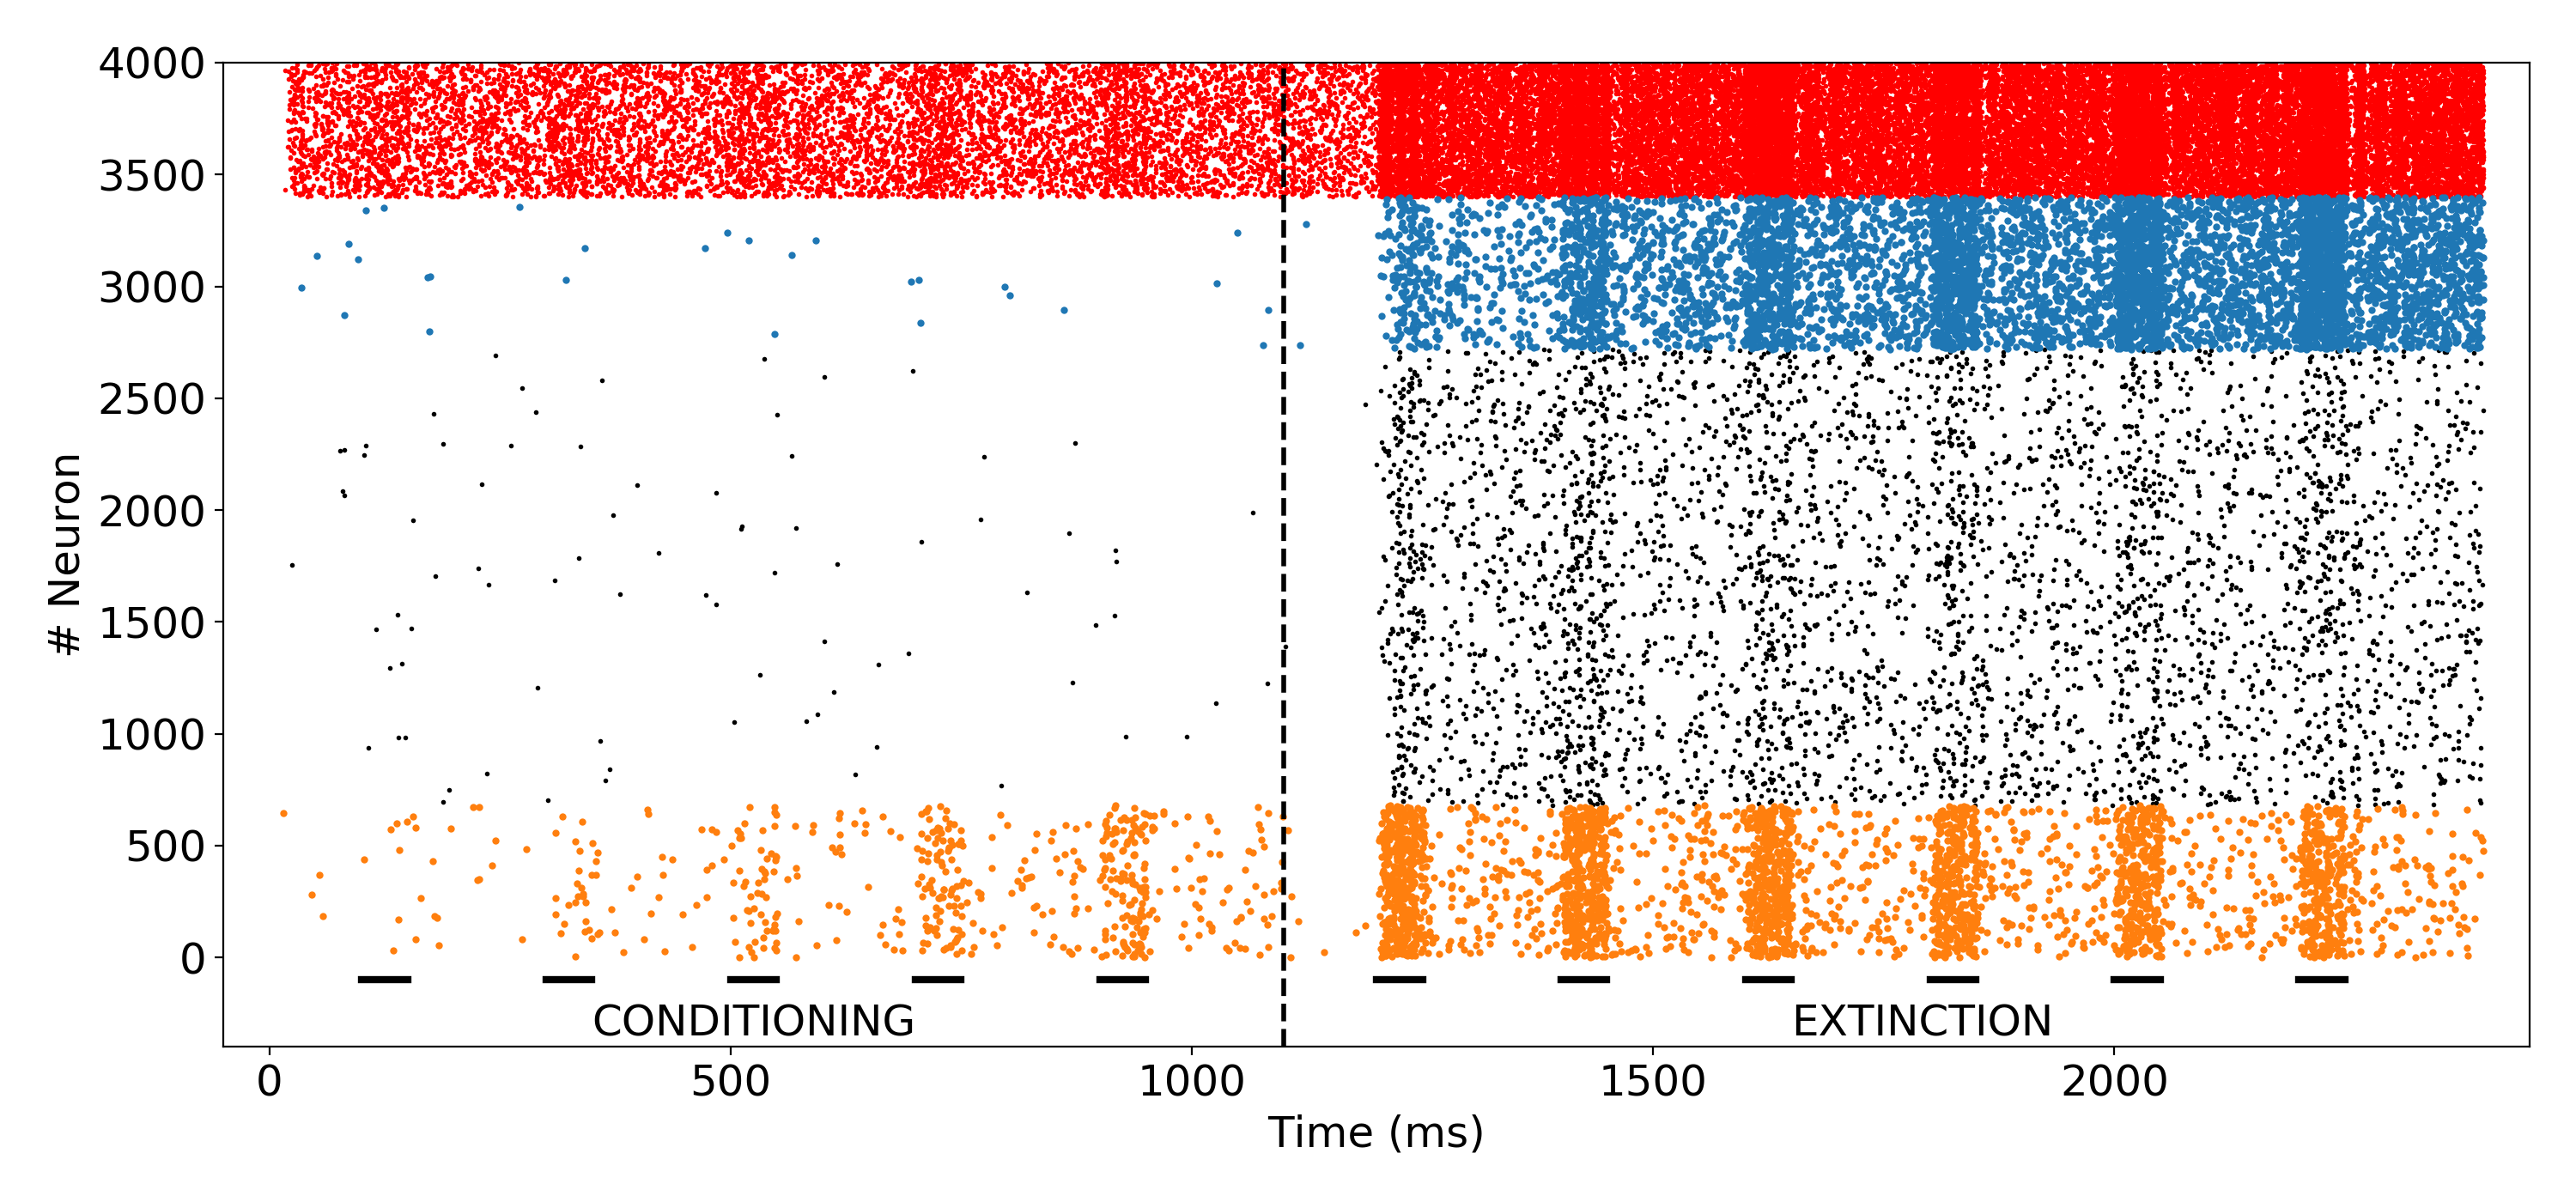
\includegraphics[width=1.0\textwidth]{figures/raster_blockage_90.0.png}
\caption{\label{fig:90block} Blockage of 90\% inhibitory activity during the extinction phase. The raster plot corresponds to the same situation (with the same color code) shown in Figure~\ref{fig:raster_COND_EXT} with the difference that in the extinction phase we set to zero the synaptic weights for 90\% of the inhibitory population. Although in our simulation these neurons fire, they do not affect other neurons.}
\end{figure}
\FloatBarrier

In Figure~\ref{fig:90block}, we show the raster plot of spiking neuronal activity for $90\%$ of inhibitory blockage. The firing rates of all excitatory neurons are abruptly increased when inhibitory neurons are deactivated during $CTX_B$ presentation. To underline this effect, in Figure~\ref{fig:gabablock} we show the firing rate during the last $CS$ presentation (corresponding to Figure 8\textbf{C} of the original paper). As expected, the increase in the fraction of ``blocked'' inhibitory cells provokes an increase in the firing rate, and this effect is even stronger for the extinction neurons ($pop_B$). This suggests that if the relative difference between the activities of the fear and extinction neurons were crucial, extinction must be favored by the blockage of inhibition in this scenario.

\begin{figure}[!ht]
\centering
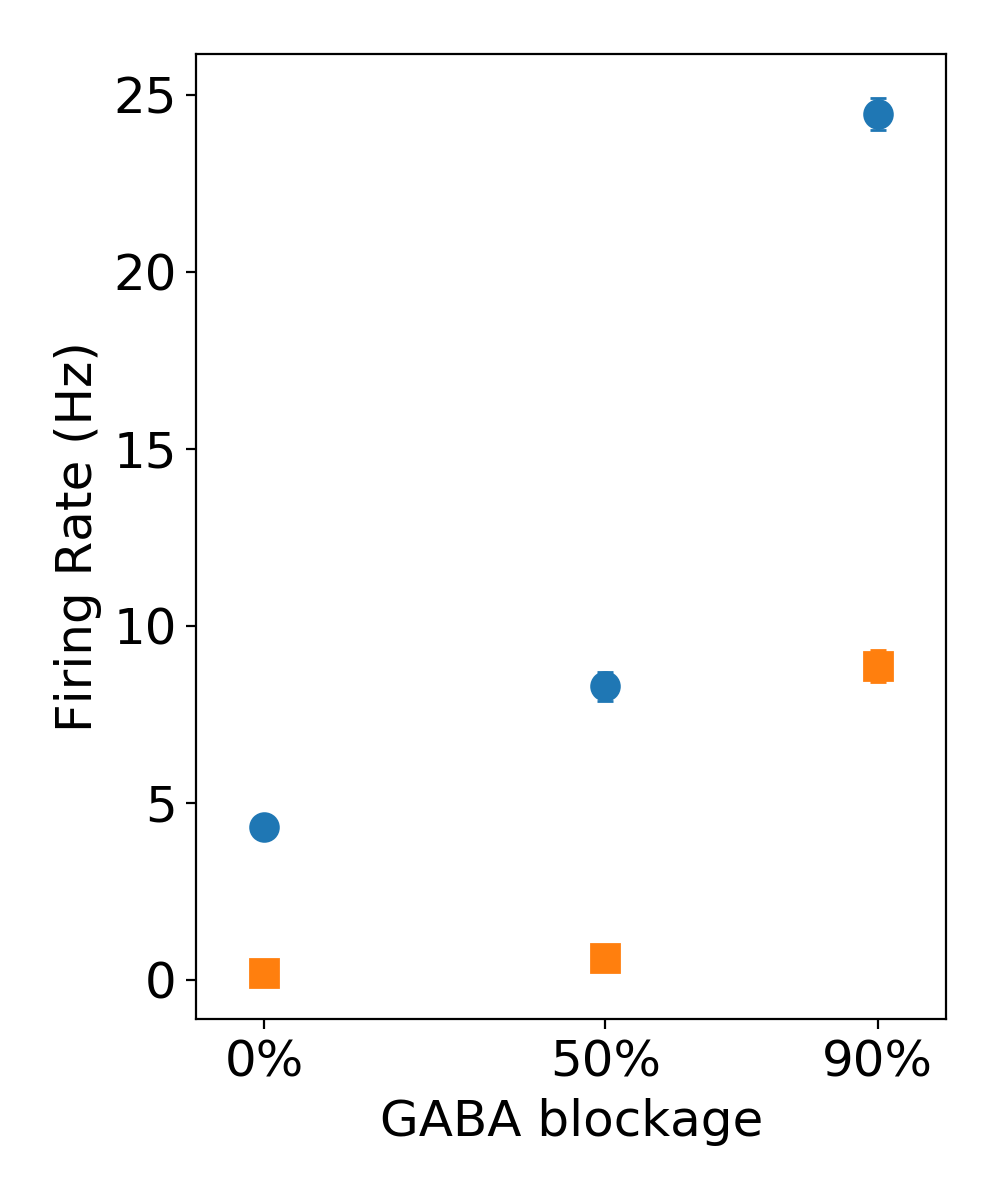
\includegraphics[width=5.5cm]{figures/gaba_block.png}
\caption{\label{fig:gabablock} Blockage of inhibitory neurons during the extinction phase leads to an increase in the firing rates of $pop_A$ (fear neurons, amber) and $pop_B$ (extinction neurons, cyan). The relative difference between the firing rates also increases.}
\end{figure}


\FloatBarrier


\section*{Conclusions}
We replicated two models proposed by Vlachos et al. (2011)~\cite{Vlachos2011} to study aspects related to fear and extinction memories in the BA. These phenomena depend on the activation of two subpopulations of neurons for different context stimuli. The models were originally built in NEST and Matlab and here we reimplemented them using Python and Brian 2.

Due to lack of some parameter values, data analysis details, and simulation protocols in the original article, we had to make some adaptations and successfully replicated the following results:
\begin{itemize}

\item for the mean-field model, the obtained result qualitatively replicates the original result. 
\item for the spiking network model, the results obtained are qualitatively consistent with the original work. In addition, we added descriptions and extra figures that help to understand all the methodological procedures adopted.
\end{itemize}

Even though we did not replicate all results of the original paper, the qualitative replication described here suffices to give support to the claim of the authors of the original article that their model captures the experimental observations.

\section*{Acknowledgements}

This replication work started as a student project during the VIII Latin American School on Computational Neuroscience (LASCON 2020).

This article was produced as part of the activities of FAPESP  Research, Innovation and Dissemination Center for Neuromathematics (Grant No. 2013$/$07699-0, S. Paulo Research Foundation). T.T.A.C. is supported by a scholarship from the National Council of Scientific and Technological Development (CNPq) (Grant No. 141579/2017-0) and Fundação de Amparo à Ciência e Tecnologia de Pernambuco (FACEPE) (Grant No. BFD-0013-1.05/20).
The authors also thank FAPESP support through Grants Nos. 2015$/$50122-0, 2018$/$20277-0  (A.C.R.), 2016$/$03855-5 (N.L.K.) and 2017$/$07688-9 (R.O.S). V.L.C received a CAPES PhD scholarship and L.B.D a Capes MSc scholarship.
A.C.R. thanks financial support from CNPq (Grant No. 306251/2014-0).
This study was financed in part by the Coordenação de Aperfeiçoamento de Pessoal de Nível Superior - Brasil (CAPES) - Finance Code 001.


